% =====================================================================================================
% Dec 5 course report: SKELETON (IEEEtran conference, 6 pages max including references).
%
% HOW TO USE
%   * Grey italic bullets (\nt{...}) are NOTES FOR YOU TO TURN INTO PROSE; delete each as you write it.
%   * Every number carries a "% SRC:" comment naming the docs/EXPERIMENTS.md section it comes from (or the script
%     that computes it). docs/report/NUMBERS.md lists them all in one table.
%   * Build:  pdflatex main && bibtex main && pdflatex main && pdflatex main      (figures are read from ../figures)
%   * \extrafigstrue (line below) turns on the optional figures; check the page count both ways.
%   * Competition rules: keep the repository and weights private until Oct 22; do not link them until then.
% =====================================================================================================
\documentclass[conference]{IEEEtran}
\usepackage{cite}
\usepackage{amsmath,amssymb}
\usepackage{graphicx}
\usepackage{booktabs}
\usepackage{array}
\usepackage{xcolor}
\usepackage{url}
\usepackage{comment}
% Notes are wrapped in a 'notes' environment: build with notes hidden to see how much room the figures, tables and
% references leave for prose:   pdflatex "\def\hidenotes{}% =====================================================================================================
% Dec 5 course report: SKELETON (IEEEtran conference, 6 pages max including references).
%
% HOW TO USE
%   * Grey italic bullets (\nt{...}) are NOTES FOR YOU TO TURN INTO PROSE; delete each as you write it.
%   * Every number carries a "% SRC:" comment naming the docs/EXPERIMENTS.md section it comes from (or the script
%     that computes it). docs/report/NUMBERS.md lists them all in one table.
%   * Build:  pdflatex main && bibtex main && pdflatex main && pdflatex main      (figures are read from ../figures)
%   * \extrafigstrue (line below) turns on the optional figures; check the page count both ways.
%   * Competition rules: keep the repository and weights private until Oct 22; do not link them until then.
% =====================================================================================================
\documentclass[conference]{IEEEtran}
\usepackage{cite}
\usepackage{amsmath,amssymb}
\usepackage{graphicx}
\usepackage{booktabs}
\usepackage{array}
\usepackage{xcolor}
\usepackage{url}
\usepackage{comment}
% Notes are wrapped in a 'notes' environment: build with notes hidden to see how much room the figures, tables and
% references leave for prose:   pdflatex "\def\hidenotes{}% =====================================================================================================
% Dec 5 course report: SKELETON (IEEEtran conference, 6 pages max including references).
%
% HOW TO USE
%   * Grey italic bullets (\nt{...}) are NOTES FOR YOU TO TURN INTO PROSE; delete each as you write it.
%   * Every number carries a "% SRC:" comment naming the docs/EXPERIMENTS.md section it comes from (or the script
%     that computes it). docs/report/NUMBERS.md lists them all in one table.
%   * Build:  pdflatex main && bibtex main && pdflatex main && pdflatex main      (figures are read from ../figures)
%   * \extrafigstrue (line below) turns on the optional figures; check the page count both ways.
%   * Competition rules: keep the repository and weights private until Oct 22; do not link them until then.
% =====================================================================================================
\documentclass[conference]{IEEEtran}
\usepackage{cite}
\usepackage{amsmath,amssymb}
\usepackage{graphicx}
\usepackage{booktabs}
\usepackage{array}
\usepackage{xcolor}
\usepackage{url}
\usepackage{comment}
% Notes are wrapped in a 'notes' environment: build with notes hidden to see how much room the figures, tables and
% references leave for prose:   pdflatex "\def\hidenotes{}% =====================================================================================================
% Dec 5 course report: SKELETON (IEEEtran conference, 6 pages max including references).
%
% HOW TO USE
%   * Grey italic bullets (\nt{...}) are NOTES FOR YOU TO TURN INTO PROSE; delete each as you write it.
%   * Every number carries a "% SRC:" comment naming the docs/EXPERIMENTS.md section it comes from (or the script
%     that computes it). docs/report/NUMBERS.md lists them all in one table.
%   * Build:  pdflatex main && bibtex main && pdflatex main && pdflatex main      (figures are read from ../figures)
%   * \extrafigstrue (line below) turns on the optional figures; check the page count both ways.
%   * Competition rules: keep the repository and weights private until Oct 22; do not link them until then.
% =====================================================================================================
\documentclass[conference]{IEEEtran}
\usepackage{cite}
\usepackage{amsmath,amssymb}
\usepackage{graphicx}
\usepackage{booktabs}
\usepackage{array}
\usepackage{xcolor}
\usepackage{url}
\usepackage{comment}
% Notes are wrapped in a 'notes' environment: build with notes hidden to see how much room the figures, tables and
% references leave for prose:   pdflatex "\def\hidenotes{}\input{main.tex}"
\ifdefined\hidenotes\excludecomment{notes}\else\includecomment{notes}\fi
\graphicspath{{../figures/}}

\newcommand{\nt}[1]{\textcolor{gray}{\textit{#1}}}            % note-to-self (replace with prose)
\newcommand{\todo}[1]{\textcolor{red}{\textbf{[TODO: #1]}}}
\newif\ifextrafigs
\extrafigsfalse   % set \extrafigstrue to include the optional figures (OOF ROC, slot-share heat map)

\begin{document}

\title{Weak Supervision and Window-Level Attention for Knee-MRI Abnormality Detection:\\
Lessons from the RSNA 2026 Kaggle Challenge}   % working title

\author{\IEEEauthorblockN{Husnain Rasool}
\IEEEauthorblockA{\textit{[Department / course]} \\
\textit{[University]} \\
\textit{[email]}}}

\maketitle

\begin{abstract}
\nt{150--200 words. Must say: (1) 12 knee-MRI findings, macro ROC-AUC, only 58 of 4,407 training studies have
image-review labels, the rest have free-text reports (not available at test time); (2) a report-to-label engine
(two open LLMs, calibrated on the 58); (3) the DINOv2 slot model plateaued near 0.89 public AUC, a window-level
attention model reached 0.929 (the change bundled four things, none isolated); (4) the final model is a 10-checkpoint
ensemble of that model; a 2-fold version runs in about 20 minutes; (5) what was learned about validation and about
silent runtime fallbacks. Numbers: 0.893 $\rightarrow$ 0.929 public LB; OOF 0.8840; gold-58 0.9111.}
\end{abstract}

\begin{IEEEkeywords}
knee MRI, weak supervision, multiple-instance learning, attention, Kaggle, evaluation methodology
\end{IEEEkeywords}

% ======================================================================================================
\section{Introduction}
\begin{notes}
\begin{itemize}
\item \nt{The task: 12 binary findings per knee-MRI study (ACL, MCL, medial/lateral meniscus, three OA compartments,
effusion, synovitis, Baker's cyst, contusion, fracture); metric = macro-averaged ROC-AUC; Kaggle code competition
(GPU $\le$ 9 h, no internet), $\sim$1,300 hidden test studies.}  % SRC: CLAUDE.md s1
\item \nt{The difficulty is the supervision: 4,407 training studies, 58 with image-review labels, every study with a
radiology report in 12+ languages, no reports at test time; reports agree with image review only $\sim$82\%
(they over-call mild disease).}  % SRC: CLAUDE.md s2
\item \nt{Contributions, kept honest: (i) a report-to-label engine calibrated on 58 studies; (ii) a diagnosis of a
$\sim$0.89 plateau and a window-level attention model that scored 0.929 public (a bundled change, not an ablation);
(iii) a measurement-discipline thread: pre-registered bars, paired cluster bootstrap, runtime measured on the target
hardware, and the discovery that a runtime fallback silently changed which model was scored.}
\item \nt{State the scope limits early: public leaderboard only (private rank known Oct 22); gold set is $n=58$.}
\end{itemize}
\end{notes}

\section{Related Work}
\begin{notes}
\begin{itemize}
\item \nt{Public knee MRI benchmarks: MRNet~\cite{bien2018mrnet} (not used: licensing; no external data used).}
\item \nt{Report-derived labels: rule/LLM labelers for radiology reports, e.g. CheXpert~\cite{irvin2019chexpert}; here the
labeler is a rubric-conditioned open LLM calibrated on a tiny gold set.}
\item \nt{Noisy-student self-training~\cite{xie2020noisystudent} (used once: image-model out-of-fold predictions blended
back into the labels; a second round regressed).}
\item \nt{Attention-based multiple-instance learning~\cite{ilse2018attention}; backbones DINOv2~\cite{oquab2023dinov2} and
CoAtNet~\cite{dai2021coatnet} via timm~\cite{wightman2019timm}.}
\item \nt{The window-MIL design follows a public Kaggle kernel~\cite{dread2026kernel}; say so plainly (re-implemented, own
labels and folds, no third-party weights or labels).}
\item \nt{LLM tooling: Qwen2.5~\cite{qwen2025}, Llama~3~\cite{llama3}, vLLM~\cite{kwon2023vllm}.}
\item \todo{add the external published benchmark noted in EXPERIMENTS.md 2026-09-17 (``Qiu et al. 2024, Nat Commun''):
its title and DOI are not recorded in the repo.}
\end{itemize}
\end{notes}

\section{Data and Task}
\begin{notes}
\begin{itemize}
\item \nt{4,407 training studies, 24,371 series (mean 5.53 per study, range 3--14; sagittal 9,864, coronal 8,609,
axial 5,898); mixed DICOM transfer syntaxes (JPEG Lossless, JPEG 2000).}  % SRC: CLAUDE.md s3
\item \nt{Gold-58 positive rates (ACL .41 ... Effusion .60) show the label shift risk; test prevalence unknown.}
  % SRC: CLAUDE.md s3
\item \nt{Validation protocol: 5-fold GroupKFold over report-template clusters (3,681 clusters); gold-58 never trained
on; OOF macro-AUC against the report-derived proxy labels is the main selection signal, gold-58 a tripwire, public LB the
external check.}  % SRC: EXPERIMENTS.md 2026-09-20 results block (3,681 clusters)
\item \nt{Noise scale: paired cluster bootstrap SD of a solo macro-AUC $\approx 0.0041$, so 2 SD $=0.0082$ was the
pre-registered bar for ablations.}  % SRC: EXPERIMENTS.md ablation ledger conventions
\end{itemize}
\end{notes}

\section{Label Engine}
\begin{notes}
\begin{itemize}
\item \nt{Two open LLMs (Qwen2.5-72B-Instruct, Llama-3.3-70B) read each report against a per-finding rubric that encodes
the experts' severity thresholds (``on the fence'' = negative); structured output per finding.}
\item \nt{Per-label strategy (Qwen / Llama / blend) chosen by strict leave-one-out AUC on gold-58: macro LOO 0.823
(\texttt{labels\_v2\_final}); report-vs-gold agreement $\sim$82\%.}  % SRC: ledger LE3
\item \nt{Noisy-student round (\texttt{labels\_v3}): blend with an image model's out-of-fold predictions, weight per label
by LOO: chosen-blend LOO 0.904; accepted by a two-criterion test (OOF vs original labels 0.8631 vs 0.8489, gold-58
+0.0139). A second round (v4) regressed ($-0.012$ LOO) and was stopped.}  % SRC: ledger LE4, LE5
\item \nt{Effect of labels alone: +0.0142 OOF at fixed architecture (exp005 vs exp002).}  % SRC: ledger B
\end{itemize}
\end{notes}

\section{Image Models}
\begin{figure*}[t]   % PLACEMENT: top of the page where section V starts; full width
\centering
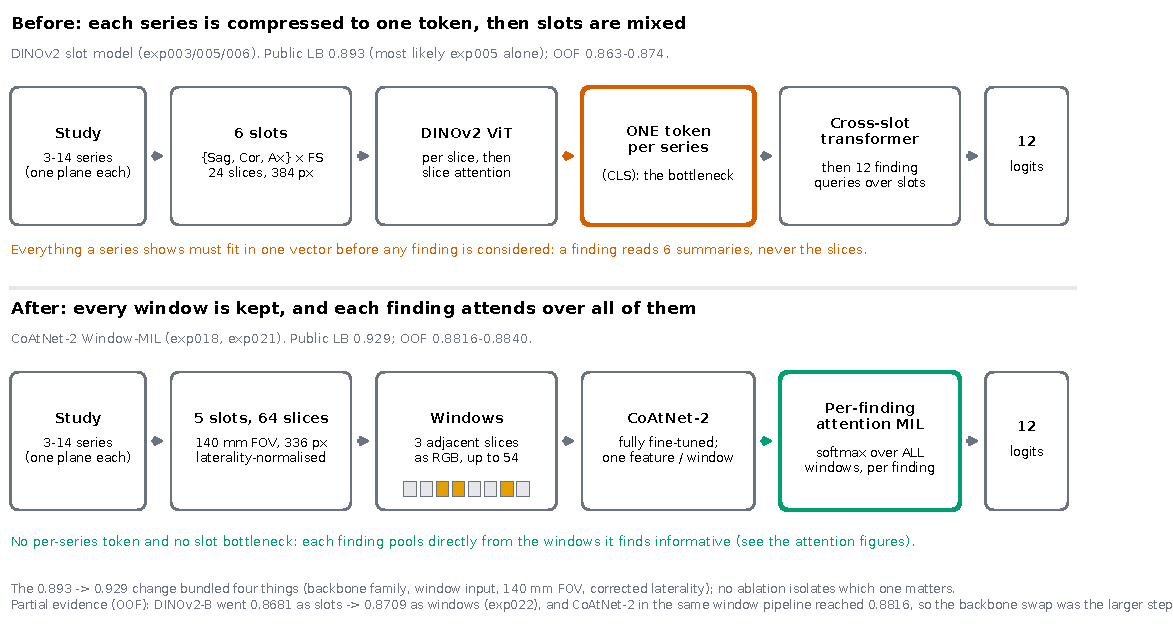
\includegraphics[width=0.97\textwidth]{formulation_before_after.pdf}
\caption{Series-token compression (DINOv2 slot model) versus per-finding window attention (CoAtNet-2 Window-MIL).
The 0.893 $\rightarrow$ 0.929 change bundled four things (backbone family, window input, 140~mm FOV, corrected
laterality); no ablation isolates which one matters.}
\label{fig:formulation}
\end{figure*}
\subsection{Slot model (first formulation)}
\begin{notes}
\begin{itemize}
\item \nt{DINOv2 ViT per slice (24 slices, 384 px) $\rightarrow$ slice-attention transformer $\rightarrow$ one CLS token per
series $\rightarrow$ 6 slots \{sag, cor, ax\}$\times$\{fluid-sensitive or not\} $\rightarrow$ cross-slot transformer $\rightarrow$
12 per-finding queries.}  % SRC: README.md "How it works" 3; src/rsna_knee/model.py
\item \nt{OOF: ViT-S 0.8631 (v3 labels), ViT-B 0.8681, 3-member ensemble 0.8744.}  % SRC: ledger B
\end{itemize}
\end{notes}
\subsection{Window-MIL (final formulation)}
\begin{notes}
\begin{itemize}
\item \nt{140~mm FOV at 336 px, 64 slices over five slots (18/14/12/8/12), laterality-normalized; windows of 3 adjacent
slices as RGB (at most 54 per study); fully fine-tuned CoAtNet-2; per-finding attention over all windows.}
  % SRC: README.md "How it works" 2; src/rsna_knee/wmil.py
\item \nt{Laterality: coronal/axial mirrored for right knees, sagittal slice order reversed; side from validated table,
then DICOM tag, then an image-centre geometry rule (99.4\% of the 1,491 studies previously un-normalized; 99.0--99.1\%
agreement).}  % SRC: METHOD_WRITEUP s5a; exp018_cache_audit.md
\item \nt{Training: top-3 epoch weight averaging; labels v3; pre-registered fold-0 kill rule (gold-58 $<$ 0.880).}
\item \nt{Final main model: exp021 = 10 checkpoints (seed 42 and 43, five folds each, probability mean). Efficiency model:
exp018 folds 0--1 only.}
\end{itemize}
\end{notes}
\subsection{Evaluation and efficiency track}
\begin{notes}
\begin{itemize}
\item \nt{Efficiency score $=\text{AUC}/(0.5-\max\text{AUC}) + t/32400$ (minimised); $\max\text{AUC}=0.95$ is an
assumption here.}  % SRC: CLAUDE.md s4
\item \nt{Inference in fp16 (never bf16 on T4); two T4 GPUs; runtimes measured on Kaggle's own machine.}
\end{itemize}
\end{notes}

% ======================================================================================================
\section{Results}
\begin{table}[t]   % PLACEMENT: right after the section heading
\caption{Main results. OOF is scored against report-derived labels; gold-58 against image-review labels (fold-ensembled);
LB is the public leaderboard. Runtimes are measured on Kaggle's 2$\times$T4 for $\sim$1,300 studies.}
\label{tab:main}
\centering\footnotesize
\begin{tabular}{@{}p{2.55cm}cccc@{}}
\toprule
Model & OOF & Gold-58 & LB & Time \\
\midrule
DINOv2 slot pipeline$^{a}$ & 0.8631 & 0.8903 & 0.893 & --- \\  % SRC: 2026-10-01 re-gate (exp005 0.8631/0.8903); 0.893 LB
Distilled DINOv2-S$^{b}$ & 0.8708 & 0.888 & 0.885 & --- \\       % SRC: ledger B (exp008 0.8708/0.8882); METHOD_WRITEUP s11 (0.885)
Window-MIL, 5 folds (exp018) & 0.8816 & 0.9091 & 0.929 & $\sim$53 min \\   % SRC: 2026-09-21 result; 2026-09-26 profile
Window-MIL, 10 ckpt (exp021) & \textbf{0.8840} & \textbf{0.9111} & \textbf{0.929} & $\sim$100 min \\ % SRC: 2026-09-25
Window-MIL, 2 folds & n/a & 0.9078 & 0.925 & $\sim$20.5 min \\     % SRC: README.md results; 2026-09-26 probes #5/#6
\bottomrule
\end{tabular}\\[2pt]
{\footnotesize $^{a}$Most likely exp005 alone after the notebook's runtime fallback (inferred; the 3-member ensemble
measures $\sim$21~h on T4). $^{b}$Fold count chosen at run time; the scored count is unknown.}
\end{table}
\begin{notes}
\begin{itemize}
\item \nt{Say the 0.893 attribution here (see Limitations): the notebook chooses its configuration from a time budget.}
\item \nt{exp021 over exp018: OOF +0.0024, 95\% paired CI [+0.0014, +0.0033]; gold-58 +0.0021 (CI spans zero).}
  % SRC: EXPERIMENTS.md 2026-09-25
\item \nt{Leaderboard beat OOF every time: about +0.030 (slot pipeline, corrected), +0.047 (exp018); OOF is scored against
noisy report labels.}  % SRC: 2026-10-01 correction; 2026-09-22
\end{itemize}
\end{notes}

\begin{figure*}[t]   % PLACEMENT: top of the next page
\centering
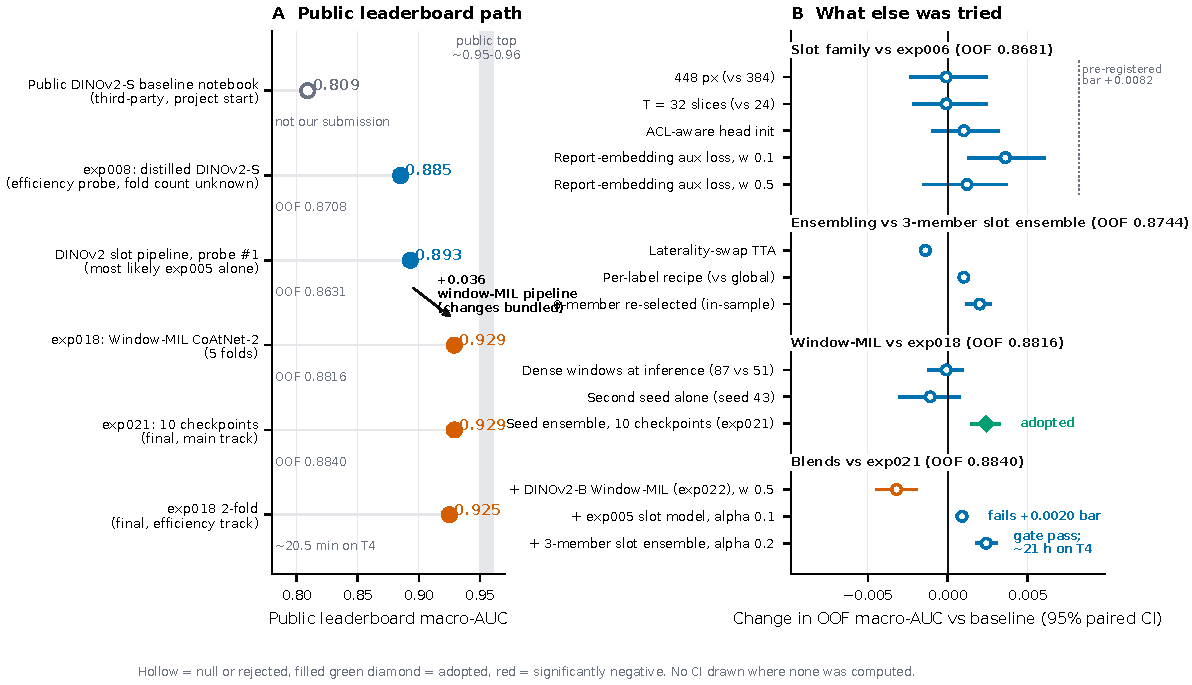
\includegraphics[width=0.93\textwidth]{ablation_path_and_nulls.pdf}
\caption{(A) Public leaderboard path (the 0.809 baseline is a third-party notebook, not a submission). (B) Every tested
change as a paired OOF delta with its 95\% cluster-bootstrap interval, grouped by baseline.}
\label{fig:ablation}
\end{figure*}

\begin{table*}[t]   % PLACEMENT: after Fig. 2; filled from docs/EXPERIMENTS.md (section per row in the SRC comments)
\caption{Ablation ledger. $\Delta$ is OOF macro-AUC against the stated baseline; intervals are paired cluster bootstrap
over 3,681 report clusters unless noted. ``Bar'' is the pre-registered $+0.0082$ for the slot family.}
\label{tab:ablation}
\centering\footnotesize
\begin{tabular}{@{}llccl@{}}
\toprule
Change & Baseline (OOF) & $\Delta$ OOF & 95\% CI & Verdict \\
\midrule
448 px (vs 384) & exp006 (0.8681) & $-0.0001$ & [$-0.0024$, $+0.0025$] & null \\          % SRC: ledger C, exp015
$T=32$ slices (vs 24) & exp006 & $-0.0001$ & [$-0.0022$, $+0.0025$] & null \\              % SRC: ledger C, exp010
ACL-aware head init & exp006 & $+0.0010$ & [$-0.0010$, $+0.0032$] & null (MCL $-0.0122$) \\ % SRC: 2026-09-20 block, exp012
Report-embedding aux loss, $w=0.1$ & exp006 & $+0.0036$ & [$+0.0012$, $+0.0061$] & below bar \\ % SRC: ledger C, exp016a
Report-embedding aux loss, $w=0.5$ & exp006 & $+0.0012$ & [$-0.0016$, $+0.0037$] & null \\ % SRC: ledger C, exp016b
Laterality-swap TTA & 3-member (0.8744) & $-0.0014$ & --- & rejected \\               % SRC: ledger D
Per-label ensemble recipe & 3-member & $+0.0010$ & --- & below $0.002$ bar \\          % SRC: ledger D
6-member re-selected ensemble & 3-member & $+0.0020$ & [$+0.0011$, $+0.0027$] & in-sample; $2.9\times$ cost \\ % SRC: ledger D
Dense windows at inference (87 vs 51) & exp018 (0.8816) & $-0.0001$ & [$-0.0013$, $+0.0010$] & null \\ % SRC: 2026-09-26 dense
Second seed alone (seed 43) & exp018 & $-0.0011$ & [$-0.0031$, $+0.0008$] & null \\       % SRC: 2026-09-25 exp021
\textbf{10-checkpoint seed ensemble} & exp018 & $+0.0024$ & [$+0.0014$, $+0.0033$] & \textbf{adopted} \\ % SRC: 2026-09-25
DINOv2-B inside the window pipeline (solo) & exp018 & $-0.0107$ & --- & worse (0.8709) \\ % SRC: 2026-09-26 exp022; delta = 0.8709-0.8816
EMA, decay 0.999 (fold 0, gold-58) & top-3 average & $-0.0009$ & --- & null \\         % SRC: 2026-09-24 exp020 (fold-0 gold-58, not OOF)
+ DINOv2-B window model, $w=0.5$ & exp021 (0.8840) & $-0.0032$ & [$-0.0045$, $-0.0019$] & gate fail \\ % SRC: 2026-09-26 exp022
+ 3-member slot ensemble, $\alpha=0.2$ & exp021 & $+0.0024$ & [$+0.0017$, $+0.0031$] & gate pass; $\sim$21 h on T4 \\ % SRC: 2026-09-26 gate
+ exp005, $\alpha=0.1$ & exp021 & $+0.0009$ & [$+0.0005$, $+0.0012$] & below $+0.0020$ bar \\ % SRC: 2026-10-01 re-gate
\bottomrule
\end{tabular}
\end{table*}
\begin{notes}
\begin{itemize}
\item \nt{Write the null-result paragraph: six pre-registered slot-family changes inside noise; ViT-S$\to$ViT-B
($+0.005$), v3 labels ($+0.014$) and ensembling ($+0.006$) were the only early gains; the plateau was a property of
the model family.}  % SRC: ledger "Reading the whole record"
\item \nt{Other rejected items worth one clause: DINOv3-S ($-0.0252$), ConvNeXt-V2 (redundant, corr 0.93), 3D ResNet
(killed), CoAtNet-3 (no result: no pretrained checkpoint at the intended size, then a 32-bit indexing overflow).}
  % SRC: ledger B; 2026-09-24
\item \nt{The blend: the 3-member arm passes an offline gate but cannot run in time on T4; the single-model arm fails the
bar; modeling closed.}  % SRC: 2026-09-27, 2026-10-01
\end{itemize}
\end{notes}

\begin{table}[t]   % PLACEMENT: column width; numbers generated by scripts/report_tables.py
\caption{Per-label AUC. OOF: 4,349 studies against report-derived labels; gold-58: against image review.}
\label{tab:perlabel}
\centering\footnotesize
\begin{tabular}{@{}lcccc@{}}
\toprule
 & \multicolumn{2}{c}{OOF} & \multicolumn{2}{c}{Gold-58} \\
\cmidrule(lr){2-3}\cmidrule(lr){4-5}
Finding & exp018 & exp021 & exp018 & exp021 \\
\midrule
\input{tables/per_label_auc.tex} \\
\bottomrule
\end{tabular}
\end{table}
\begin{notes}
\begin{itemize}
\item \nt{ACL: lowest-ish on OOF (0.857) but 0.979 on gold-58, so the OOF deficit is proxy-label noise.}
  % SRC: table above; EXPERIMENTS.md 2026-09-18 ACL conclusion
\item \nt{Weakest on gold-58: PF OA 0.824, lateral OA 0.828, lateral meniscus 0.834 ($n=58$: wide intervals).}
\end{itemize}
\end{notes}

\ifextrafigs   % optional: ~0.6 page; the per-label table carries the same numbers
\begin{figure*}[t]
\centering
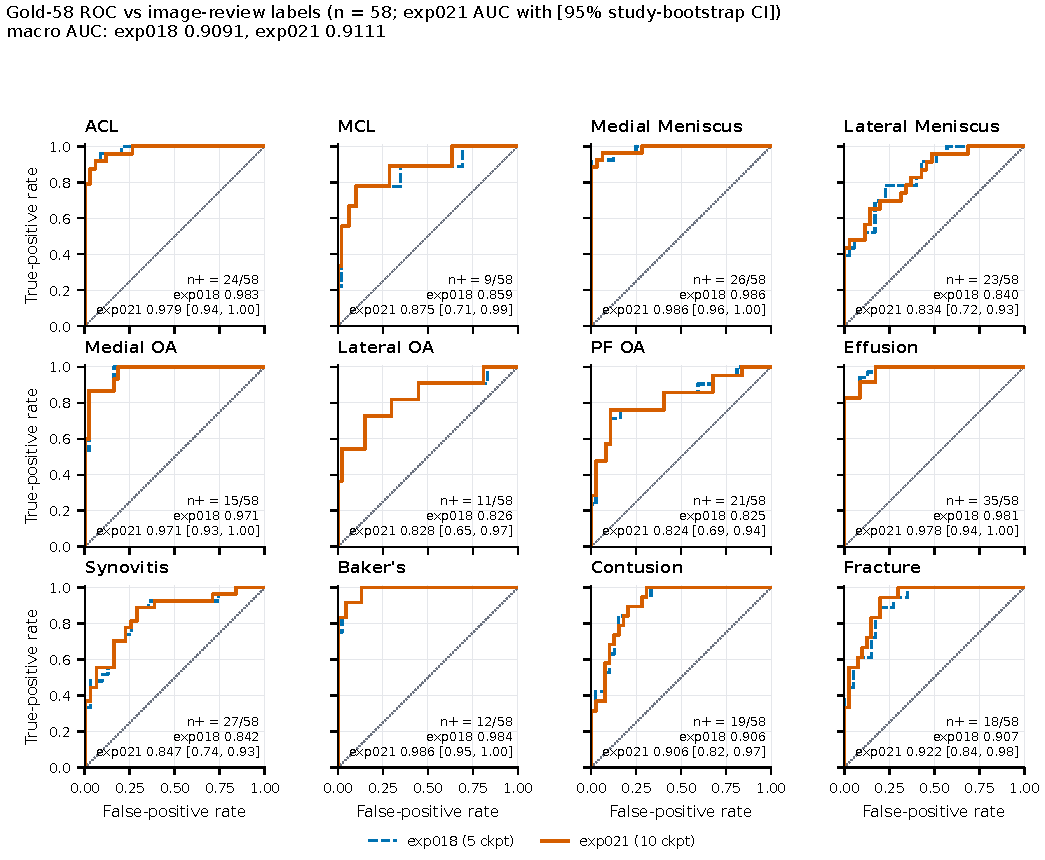
\includegraphics[width=0.93\textwidth]{roc_gold58_exp018_exp021.pdf}
\caption{Per-finding ROC curves on the 58 image-review studies (exp021 AUC with 95\% study-bootstrap interval).}
\label{fig:roc}
\end{figure*}
\begin{figure*}[t]
\centering
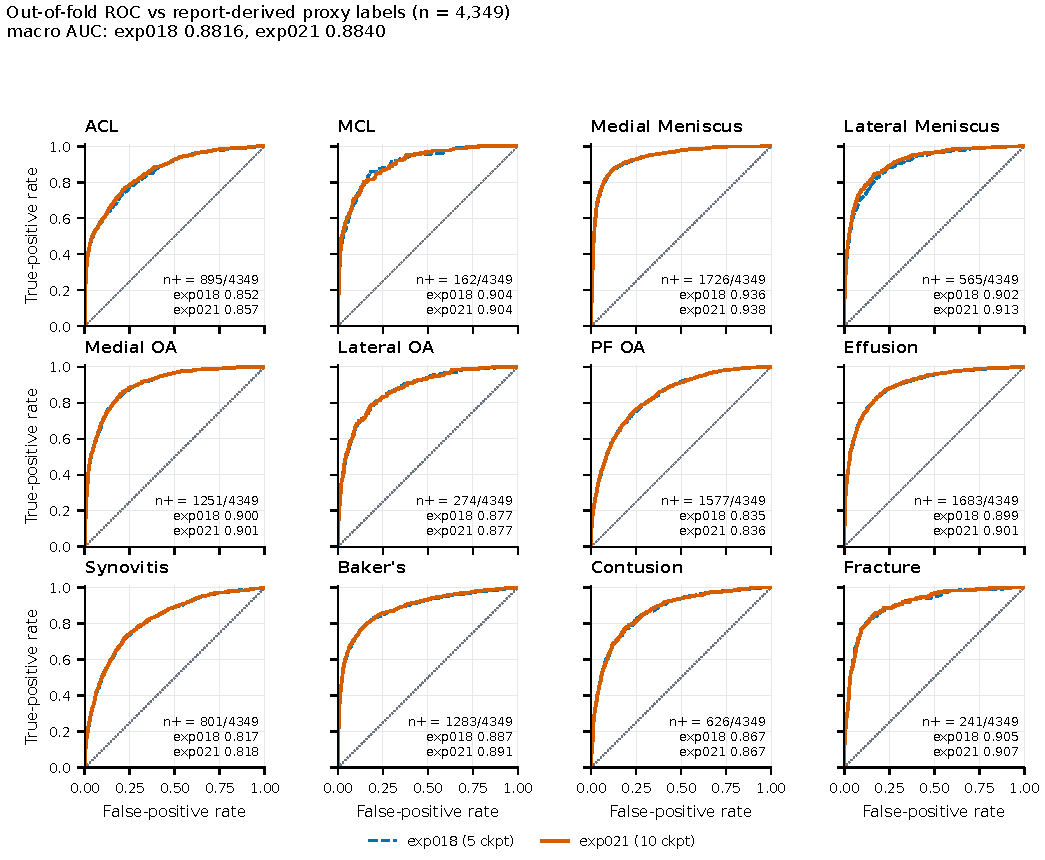
\includegraphics[width=0.93\textwidth]{roc_oof_exp018_exp021.pdf}
\caption{Out-of-fold ROC curves against report-derived labels ($n=4{,}349$).}
\label{fig:rocoof}
\end{figure*}
\fi

\begin{table}[t]
\caption{Efficiency track (maxAUC assumed 0.95; public AUC; lower is better).}
\label{tab:eff}
\centering\footnotesize
\begin{tabular}{@{}lccc@{}}
\toprule
Configuration & LB AUC & Time & Score \\
\midrule
Distilled DINOv2-S & 0.885 & $\sim$11.6 min$^{c}$ & $-1.945$ \\  % SRC: exp018_efficiency_table.md (projected runtime)
Window-MIL, 5 folds & 0.929 & $\sim$53 min & $-1.966$ \\             % SRC: computed: 0.929/(-0.45)+3180/32400
Window-MIL, 2 folds & 0.925 & $\sim$20.5 min & $\mathbf{-2.018}$ \\   % SRC: 2026-09-26 efficiency entries
\bottomrule
\end{tabular}\\[2pt]
{\footnotesize $^{c}$Projected, not measured.}
\end{table}
\begin{notes}
\begin{itemize}
\item \nt{Model-bound, not decode-bound: 5 folds take $\sim$4.5 s/study on one T4 ($\sim$53 min), so fold count is the lever;
2 folds run at the DICOM-decode floor.}  % SRC: 2026-09-26 "C" entries
\item \nt{Tested and not adopted: channels\_last ($-3.7\%$ time, predictions within $3\times10^{-4}$), 4th decode thread (no gain).}
\end{itemize}
\end{notes}

% ======================================================================================================
\section{Analysis}
\begin{figure*}[t]   % PLACEMENT: top of the page; slide variant has 3 rows (the 6-row version is attention_windows_gold58.pdf)
\centering
\includegraphics[width=0.8\textwidth]{attention_windows_gold58_slide.pdf}
\caption{Window-MIL attention (exp021, mean of 10 checkpoints) for three gold-positive studies: the four most-attended
windows and the attention over all windows. Studies were chosen by a fixed rule before any map was viewed (the most
confidently detected gold-positive study per finding); this is a best case, not a hit rate.}
\label{fig:attention}
\end{figure*}
\begin{notes}
\begin{itemize}
\item \nt{Attention view: ACL pools mostly from sagittal fat-suppressed slices, medial meniscus from coronal, Baker's cyst
from axial. Over all 58 gold studies: ACL 62\% of attention on sagittal FS (30\% if uniform), Baker's 45\% on axial (20\%
uniform), effusion 57\% sagittal FS.}  % SRC: docs/figures/attention_slot_mass_gold58.csv
\item \nt{Attention is broad: top-4 windows hold 22--48\% in the selected studies; a finding pools over about 16--40
effective windows (mean 52 windows per study).}  % SRC: same csv, column effective_windows
\item \nt{Caveat: this shows where the pooling draws from, not that it localizes the lesion; no radiologist reviewed the
windows; the two seed groups agree on window attention (per-finding Spearman 0.85--0.95).}  % SRC: csv, seed42_vs_seed43
\end{itemize}
\end{notes}
\ifextrafigs
\begin{figure}[t]
\centering
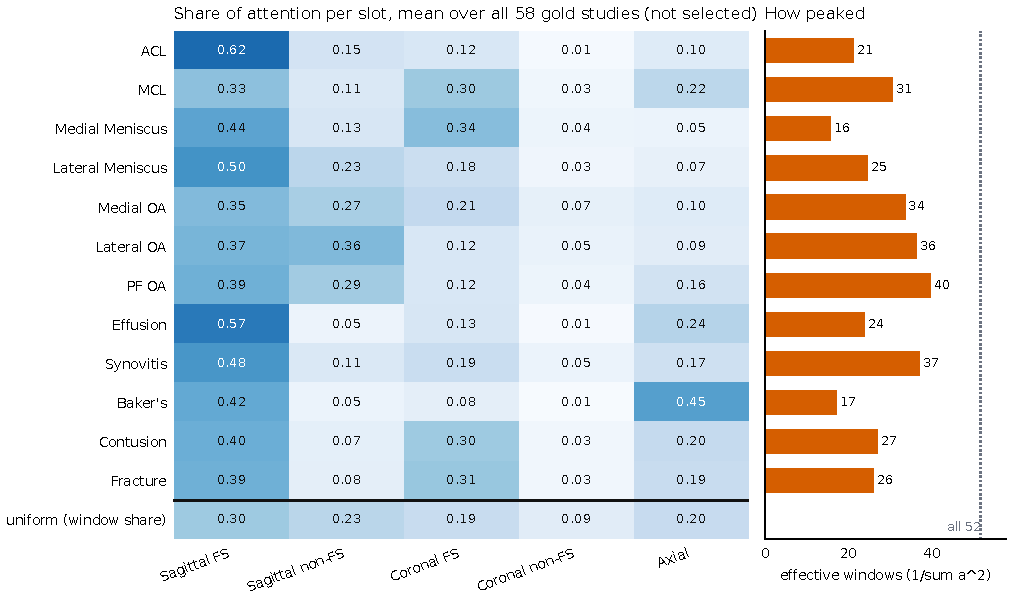
\includegraphics[width=\columnwidth]{attention_by_slot_gold58.pdf}
\caption{Share of attention per slot, all 58 gold studies (not selected), and how peaked the attention is.}
\label{fig:slotshare}
\end{figure}
\fi
\subsection{Validation lessons}
\begin{notes}
\begin{itemize}
\item \nt{OOF vs LB gaps: slot pipeline $\sim-0.030$ (0.8631 vs 0.893; first recorded as $-0.0186$ on the 3-member OOF,
corrected), exp008 $-0.014$ to $-0.020$, exp018 $-0.0474$. Reading: report-derived OOF is a conservative proxy; leakage would
push the other way.}  % SRC: 2026-10-01 correction; METHOD_WRITEUP s11
\item \nt{A runtime degradation ladder silently changed which model was scored: the 3-member notebook measures $\sim$59
s/study on T4 ($\sim$21~h), so it almost certainly ran exp005 alone (inferred, not confirmed). The efficiency notebook also
picked its fold count at run time (unknown). Log the chosen rung; measure on target hardware before trusting a score.}
  % SRC: 2026-09-27, 2026-10-01
\item \nt{Borrowed speed factors were off by 3.6$\times$ (CoAtNet) and $\sim$13$\times$ (DINOv2) between H100 and T4.}
\item \nt{Process lessons worth a sentence each: a ``root cause'' proven off-platform was not on the failing path; a timed join
silently wrote label priors; tests must assert on prediction content, not row counts.}  % SRC: METHOD_WRITEUP s9
\end{itemize}
\end{notes}

\section{Limitations}
\begin{notes}
\begin{itemize}
\item \nt{Gold-58 ($n=58$): 95\% CI about $\pm0.03$ on macro-AUC; differences below $\sim$0.02 cannot be resolved.}
\item \nt{Public leaderboard only; the final private rank is unknown until the competition closes (Oct 22).}
\item \nt{The 0.893 $\rightarrow$ 0.929 gain is not attributed to any single change; attention maps are unvalidated
by a clinician; the 0.893 attribution to exp005 is an inference.}
\item \nt{Label-engine calibration used the same 58 studies that report gold-58 AUC (leave-one-out for the labeler; the image
models never trained on them), so the labeler's own agreement numbers are optimistic.}
\item \nt{No external data; single-person project; Kaggle hardware only for inference.}
\end{itemize}
\end{notes}

\section{Conclusion}
\begin{notes}
\begin{itemize}
\item \nt{Three sentences: what worked (calibrated report labels; per-finding attention over windows; seed ensemble), what
did not (every slot-family lever; blends), and the methodological point (pre-registration, measured runtime, logged
fallbacks).}
\item \nt{Availability: code, weights and write-up to be released after Oct 22 (repository private until then). \todo{insert URL}}
\end{itemize}
\end{notes}

\section*{Acknowledgment}
\nt{Compute: university HPC cluster (H100) and Kaggle T4 notebooks. \todo{add course/instructor thanks}}

\bibliographystyle{IEEEtran}
\bibliography{refs}

\end{document}
"
\ifdefined\hidenotes\excludecomment{notes}\else\includecomment{notes}\fi
\graphicspath{{../figures/}}

\newcommand{\nt}[1]{\textcolor{gray}{\textit{#1}}}            % note-to-self (replace with prose)
\newcommand{\todo}[1]{\textcolor{red}{\textbf{[TODO: #1]}}}
\newif\ifextrafigs
\extrafigsfalse   % set \extrafigstrue to include the optional figures (OOF ROC, slot-share heat map)

\begin{document}

\title{Weak Supervision and Window-Level Attention for Knee-MRI Abnormality Detection:\\
Lessons from the RSNA 2026 Kaggle Challenge}   % working title

\author{\IEEEauthorblockN{Husnain Rasool}
\IEEEauthorblockA{\textit{[Department / course]} \\
\textit{[University]} \\
\textit{[email]}}}

\maketitle

\begin{abstract}
\nt{150--200 words. Must say: (1) 12 knee-MRI findings, macro ROC-AUC, only 58 of 4,407 training studies have
image-review labels, the rest have free-text reports (not available at test time); (2) a report-to-label engine
(two open LLMs, calibrated on the 58); (3) the DINOv2 slot model plateaued near 0.89 public AUC, a window-level
attention model reached 0.929 (the change bundled four things, none isolated); (4) the final model is a 10-checkpoint
ensemble of that model; a 2-fold version runs in about 20 minutes; (5) what was learned about validation and about
silent runtime fallbacks. Numbers: 0.893 $\rightarrow$ 0.929 public LB; OOF 0.8840; gold-58 0.9111.}
\end{abstract}

\begin{IEEEkeywords}
knee MRI, weak supervision, multiple-instance learning, attention, Kaggle, evaluation methodology
\end{IEEEkeywords}

% ======================================================================================================
\section{Introduction}
\begin{notes}
\begin{itemize}
\item \nt{The task: 12 binary findings per knee-MRI study (ACL, MCL, medial/lateral meniscus, three OA compartments,
effusion, synovitis, Baker's cyst, contusion, fracture); metric = macro-averaged ROC-AUC; Kaggle code competition
(GPU $\le$ 9 h, no internet), $\sim$1,300 hidden test studies.}  % SRC: CLAUDE.md s1
\item \nt{The difficulty is the supervision: 4,407 training studies, 58 with image-review labels, every study with a
radiology report in 12+ languages, no reports at test time; reports agree with image review only $\sim$82\%
(they over-call mild disease).}  % SRC: CLAUDE.md s2
\item \nt{Contributions, kept honest: (i) a report-to-label engine calibrated on 58 studies; (ii) a diagnosis of a
$\sim$0.89 plateau and a window-level attention model that scored 0.929 public (a bundled change, not an ablation);
(iii) a measurement-discipline thread: pre-registered bars, paired cluster bootstrap, runtime measured on the target
hardware, and the discovery that a runtime fallback silently changed which model was scored.}
\item \nt{State the scope limits early: public leaderboard only (private rank known Oct 22); gold set is $n=58$.}
\end{itemize}
\end{notes}

\section{Related Work}
\begin{notes}
\begin{itemize}
\item \nt{Public knee MRI benchmarks: MRNet~\cite{bien2018mrnet} (not used: licensing; no external data used).}
\item \nt{Report-derived labels: rule/LLM labelers for radiology reports, e.g. CheXpert~\cite{irvin2019chexpert}; here the
labeler is a rubric-conditioned open LLM calibrated on a tiny gold set.}
\item \nt{Noisy-student self-training~\cite{xie2020noisystudent} (used once: image-model out-of-fold predictions blended
back into the labels; a second round regressed).}
\item \nt{Attention-based multiple-instance learning~\cite{ilse2018attention}; backbones DINOv2~\cite{oquab2023dinov2} and
CoAtNet~\cite{dai2021coatnet} via timm~\cite{wightman2019timm}.}
\item \nt{The window-MIL design follows a public Kaggle kernel~\cite{dread2026kernel}; say so plainly (re-implemented, own
labels and folds, no third-party weights or labels).}
\item \nt{LLM tooling: Qwen2.5~\cite{qwen2025}, Llama~3~\cite{llama3}, vLLM~\cite{kwon2023vllm}.}
\item \todo{add the external published benchmark noted in EXPERIMENTS.md 2026-09-17 (``Qiu et al. 2024, Nat Commun''):
its title and DOI are not recorded in the repo.}
\end{itemize}
\end{notes}

\section{Data and Task}
\begin{notes}
\begin{itemize}
\item \nt{4,407 training studies, 24,371 series (mean 5.53 per study, range 3--14; sagittal 9,864, coronal 8,609,
axial 5,898); mixed DICOM transfer syntaxes (JPEG Lossless, JPEG 2000).}  % SRC: CLAUDE.md s3
\item \nt{Gold-58 positive rates (ACL .41 ... Effusion .60) show the label shift risk; test prevalence unknown.}
  % SRC: CLAUDE.md s3
\item \nt{Validation protocol: 5-fold GroupKFold over report-template clusters (3,681 clusters); gold-58 never trained
on; OOF macro-AUC against the report-derived proxy labels is the main selection signal, gold-58 a tripwire, public LB the
external check.}  % SRC: EXPERIMENTS.md 2026-09-20 results block (3,681 clusters)
\item \nt{Noise scale: paired cluster bootstrap SD of a solo macro-AUC $\approx 0.0041$, so 2 SD $=0.0082$ was the
pre-registered bar for ablations.}  % SRC: EXPERIMENTS.md ablation ledger conventions
\end{itemize}
\end{notes}

\section{Label Engine}
\begin{notes}
\begin{itemize}
\item \nt{Two open LLMs (Qwen2.5-72B-Instruct, Llama-3.3-70B) read each report against a per-finding rubric that encodes
the experts' severity thresholds (``on the fence'' = negative); structured output per finding.}
\item \nt{Per-label strategy (Qwen / Llama / blend) chosen by strict leave-one-out AUC on gold-58: macro LOO 0.823
(\texttt{labels\_v2\_final}); report-vs-gold agreement $\sim$82\%.}  % SRC: ledger LE3
\item \nt{Noisy-student round (\texttt{labels\_v3}): blend with an image model's out-of-fold predictions, weight per label
by LOO: chosen-blend LOO 0.904; accepted by a two-criterion test (OOF vs original labels 0.8631 vs 0.8489, gold-58
+0.0139). A second round (v4) regressed ($-0.012$ LOO) and was stopped.}  % SRC: ledger LE4, LE5
\item \nt{Effect of labels alone: +0.0142 OOF at fixed architecture (exp005 vs exp002).}  % SRC: ledger B
\end{itemize}
\end{notes}

\section{Image Models}
\begin{figure*}[t]   % PLACEMENT: top of the page where section V starts; full width
\centering
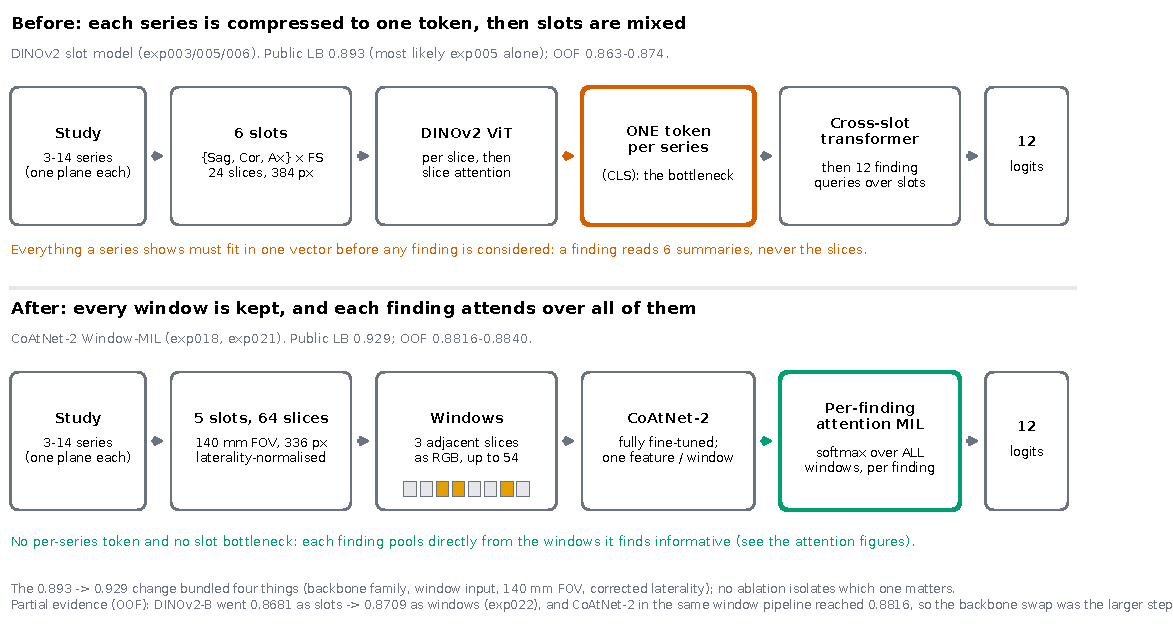
\includegraphics[width=0.97\textwidth]{formulation_before_after.pdf}
\caption{Series-token compression (DINOv2 slot model) versus per-finding window attention (CoAtNet-2 Window-MIL).
The 0.893 $\rightarrow$ 0.929 change bundled four things (backbone family, window input, 140~mm FOV, corrected
laterality); no ablation isolates which one matters.}
\label{fig:formulation}
\end{figure*}
\subsection{Slot model (first formulation)}
\begin{notes}
\begin{itemize}
\item \nt{DINOv2 ViT per slice (24 slices, 384 px) $\rightarrow$ slice-attention transformer $\rightarrow$ one CLS token per
series $\rightarrow$ 6 slots \{sag, cor, ax\}$\times$\{fluid-sensitive or not\} $\rightarrow$ cross-slot transformer $\rightarrow$
12 per-finding queries.}  % SRC: README.md "How it works" 3; src/rsna_knee/model.py
\item \nt{OOF: ViT-S 0.8631 (v3 labels), ViT-B 0.8681, 3-member ensemble 0.8744.}  % SRC: ledger B
\end{itemize}
\end{notes}
\subsection{Window-MIL (final formulation)}
\begin{notes}
\begin{itemize}
\item \nt{140~mm FOV at 336 px, 64 slices over five slots (18/14/12/8/12), laterality-normalized; windows of 3 adjacent
slices as RGB (at most 54 per study); fully fine-tuned CoAtNet-2; per-finding attention over all windows.}
  % SRC: README.md "How it works" 2; src/rsna_knee/wmil.py
\item \nt{Laterality: coronal/axial mirrored for right knees, sagittal slice order reversed; side from validated table,
then DICOM tag, then an image-centre geometry rule (99.4\% of the 1,491 studies previously un-normalized; 99.0--99.1\%
agreement).}  % SRC: METHOD_WRITEUP s5a; exp018_cache_audit.md
\item \nt{Training: top-3 epoch weight averaging; labels v3; pre-registered fold-0 kill rule (gold-58 $<$ 0.880).}
\item \nt{Final main model: exp021 = 10 checkpoints (seed 42 and 43, five folds each, probability mean). Efficiency model:
exp018 folds 0--1 only.}
\end{itemize}
\end{notes}
\subsection{Evaluation and efficiency track}
\begin{notes}
\begin{itemize}
\item \nt{Efficiency score $=\text{AUC}/(0.5-\max\text{AUC}) + t/32400$ (minimised); $\max\text{AUC}=0.95$ is an
assumption here.}  % SRC: CLAUDE.md s4
\item \nt{Inference in fp16 (never bf16 on T4); two T4 GPUs; runtimes measured on Kaggle's own machine.}
\end{itemize}
\end{notes}

% ======================================================================================================
\section{Results}
\begin{table}[t]   % PLACEMENT: right after the section heading
\caption{Main results. OOF is scored against report-derived labels; gold-58 against image-review labels (fold-ensembled);
LB is the public leaderboard. Runtimes are measured on Kaggle's 2$\times$T4 for $\sim$1,300 studies.}
\label{tab:main}
\centering\footnotesize
\begin{tabular}{@{}p{2.55cm}cccc@{}}
\toprule
Model & OOF & Gold-58 & LB & Time \\
\midrule
DINOv2 slot pipeline$^{a}$ & 0.8631 & 0.8903 & 0.893 & --- \\  % SRC: 2026-10-01 re-gate (exp005 0.8631/0.8903); 0.893 LB
Distilled DINOv2-S$^{b}$ & 0.8708 & 0.888 & 0.885 & --- \\       % SRC: ledger B (exp008 0.8708/0.8882); METHOD_WRITEUP s11 (0.885)
Window-MIL, 5 folds (exp018) & 0.8816 & 0.9091 & 0.929 & $\sim$53 min \\   % SRC: 2026-09-21 result; 2026-09-26 profile
Window-MIL, 10 ckpt (exp021) & \textbf{0.8840} & \textbf{0.9111} & \textbf{0.929} & $\sim$100 min \\ % SRC: 2026-09-25
Window-MIL, 2 folds & n/a & 0.9078 & 0.925 & $\sim$20.5 min \\     % SRC: README.md results; 2026-09-26 probes #5/#6
\bottomrule
\end{tabular}\\[2pt]
{\footnotesize $^{a}$Most likely exp005 alone after the notebook's runtime fallback (inferred; the 3-member ensemble
measures $\sim$21~h on T4). $^{b}$Fold count chosen at run time; the scored count is unknown.}
\end{table}
\begin{notes}
\begin{itemize}
\item \nt{Say the 0.893 attribution here (see Limitations): the notebook chooses its configuration from a time budget.}
\item \nt{exp021 over exp018: OOF +0.0024, 95\% paired CI [+0.0014, +0.0033]; gold-58 +0.0021 (CI spans zero).}
  % SRC: EXPERIMENTS.md 2026-09-25
\item \nt{Leaderboard beat OOF every time: about +0.030 (slot pipeline, corrected), +0.047 (exp018); OOF is scored against
noisy report labels.}  % SRC: 2026-10-01 correction; 2026-09-22
\end{itemize}
\end{notes}

\begin{figure*}[t]   % PLACEMENT: top of the next page
\centering
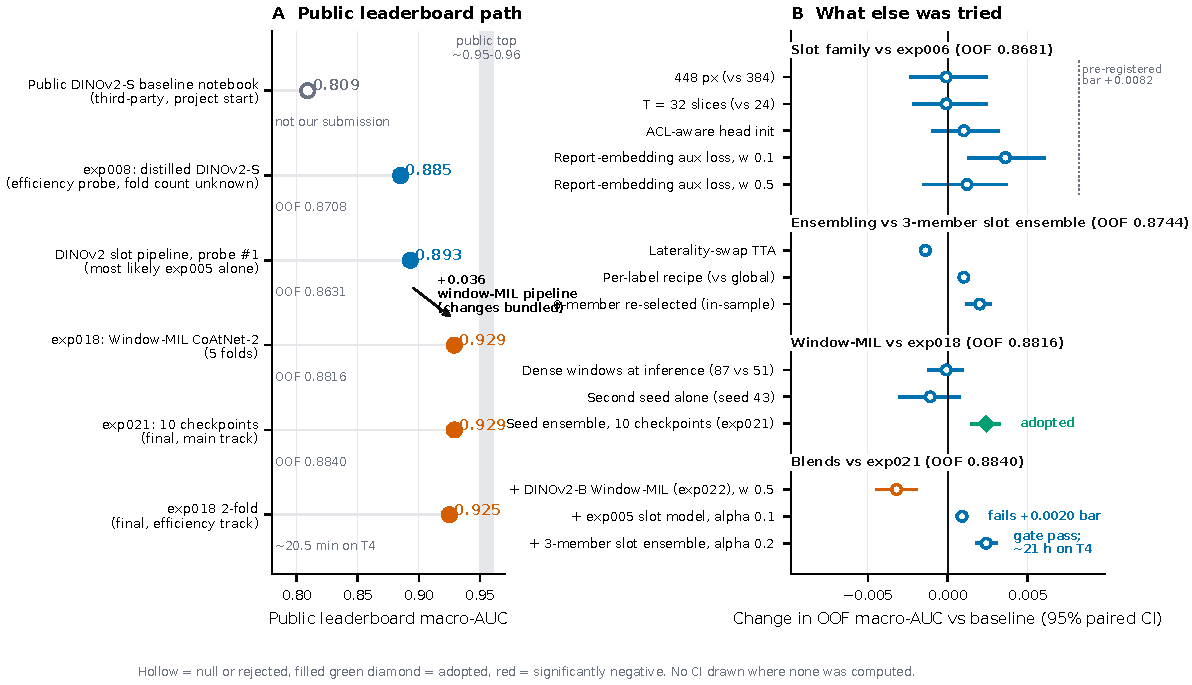
\includegraphics[width=0.93\textwidth]{ablation_path_and_nulls.pdf}
\caption{(A) Public leaderboard path (the 0.809 baseline is a third-party notebook, not a submission). (B) Every tested
change as a paired OOF delta with its 95\% cluster-bootstrap interval, grouped by baseline.}
\label{fig:ablation}
\end{figure*}

\begin{table*}[t]   % PLACEMENT: after Fig. 2; filled from docs/EXPERIMENTS.md (section per row in the SRC comments)
\caption{Ablation ledger. $\Delta$ is OOF macro-AUC against the stated baseline; intervals are paired cluster bootstrap
over 3,681 report clusters unless noted. ``Bar'' is the pre-registered $+0.0082$ for the slot family.}
\label{tab:ablation}
\centering\footnotesize
\begin{tabular}{@{}llccl@{}}
\toprule
Change & Baseline (OOF) & $\Delta$ OOF & 95\% CI & Verdict \\
\midrule
448 px (vs 384) & exp006 (0.8681) & $-0.0001$ & [$-0.0024$, $+0.0025$] & null \\          % SRC: ledger C, exp015
$T=32$ slices (vs 24) & exp006 & $-0.0001$ & [$-0.0022$, $+0.0025$] & null \\              % SRC: ledger C, exp010
ACL-aware head init & exp006 & $+0.0010$ & [$-0.0010$, $+0.0032$] & null (MCL $-0.0122$) \\ % SRC: 2026-09-20 block, exp012
Report-embedding aux loss, $w=0.1$ & exp006 & $+0.0036$ & [$+0.0012$, $+0.0061$] & below bar \\ % SRC: ledger C, exp016a
Report-embedding aux loss, $w=0.5$ & exp006 & $+0.0012$ & [$-0.0016$, $+0.0037$] & null \\ % SRC: ledger C, exp016b
Laterality-swap TTA & 3-member (0.8744) & $-0.0014$ & --- & rejected \\               % SRC: ledger D
Per-label ensemble recipe & 3-member & $+0.0010$ & --- & below $0.002$ bar \\          % SRC: ledger D
6-member re-selected ensemble & 3-member & $+0.0020$ & [$+0.0011$, $+0.0027$] & in-sample; $2.9\times$ cost \\ % SRC: ledger D
Dense windows at inference (87 vs 51) & exp018 (0.8816) & $-0.0001$ & [$-0.0013$, $+0.0010$] & null \\ % SRC: 2026-09-26 dense
Second seed alone (seed 43) & exp018 & $-0.0011$ & [$-0.0031$, $+0.0008$] & null \\       % SRC: 2026-09-25 exp021
\textbf{10-checkpoint seed ensemble} & exp018 & $+0.0024$ & [$+0.0014$, $+0.0033$] & \textbf{adopted} \\ % SRC: 2026-09-25
DINOv2-B inside the window pipeline (solo) & exp018 & $-0.0107$ & --- & worse (0.8709) \\ % SRC: 2026-09-26 exp022; delta = 0.8709-0.8816
EMA, decay 0.999 (fold 0, gold-58) & top-3 average & $-0.0009$ & --- & null \\         % SRC: 2026-09-24 exp020 (fold-0 gold-58, not OOF)
+ DINOv2-B window model, $w=0.5$ & exp021 (0.8840) & $-0.0032$ & [$-0.0045$, $-0.0019$] & gate fail \\ % SRC: 2026-09-26 exp022
+ 3-member slot ensemble, $\alpha=0.2$ & exp021 & $+0.0024$ & [$+0.0017$, $+0.0031$] & gate pass; $\sim$21 h on T4 \\ % SRC: 2026-09-26 gate
+ exp005, $\alpha=0.1$ & exp021 & $+0.0009$ & [$+0.0005$, $+0.0012$] & below $+0.0020$ bar \\ % SRC: 2026-10-01 re-gate
\bottomrule
\end{tabular}
\end{table*}
\begin{notes}
\begin{itemize}
\item \nt{Write the null-result paragraph: six pre-registered slot-family changes inside noise; ViT-S$\to$ViT-B
($+0.005$), v3 labels ($+0.014$) and ensembling ($+0.006$) were the only early gains; the plateau was a property of
the model family.}  % SRC: ledger "Reading the whole record"
\item \nt{Other rejected items worth one clause: DINOv3-S ($-0.0252$), ConvNeXt-V2 (redundant, corr 0.93), 3D ResNet
(killed), CoAtNet-3 (no result: no pretrained checkpoint at the intended size, then a 32-bit indexing overflow).}
  % SRC: ledger B; 2026-09-24
\item \nt{The blend: the 3-member arm passes an offline gate but cannot run in time on T4; the single-model arm fails the
bar; modeling closed.}  % SRC: 2026-09-27, 2026-10-01
\end{itemize}
\end{notes}

\begin{table}[t]   % PLACEMENT: column width; numbers generated by scripts/report_tables.py
\caption{Per-label AUC. OOF: 4,349 studies against report-derived labels; gold-58: against image review.}
\label{tab:perlabel}
\centering\footnotesize
\begin{tabular}{@{}lcccc@{}}
\toprule
 & \multicolumn{2}{c}{OOF} & \multicolumn{2}{c}{Gold-58} \\
\cmidrule(lr){2-3}\cmidrule(lr){4-5}
Finding & exp018 & exp021 & exp018 & exp021 \\
\midrule
ACL & 0.852 & 0.857 & 0.983 & 0.979 \\
MCL & 0.904 & 0.904 & 0.859 & 0.875 \\
Medial Meniscus & 0.936 & 0.938 & 0.986 & 0.986 \\
Lateral Meniscus & 0.902 & 0.913 & 0.840 & 0.834 \\
Medial OA & 0.900 & 0.901 & 0.971 & 0.971 \\
Lateral OA & 0.877 & 0.877 & 0.826 & 0.828 \\
PF OA & 0.835 & 0.836 & 0.825 & 0.824 \\
Effusion & 0.899 & 0.901 & 0.981 & 0.978 \\
Synovitis & 0.817 & 0.818 & 0.842 & 0.847 \\
Baker's & 0.887 & 0.891 & 0.984 & 0.986 \\
Contusion & 0.867 & 0.867 & 0.906 & 0.906 \\
Fracture & 0.905 & 0.907 & 0.907 & 0.922 \\
\midrule
Macro & 0.8816 & 0.8840 & 0.9091 & 0.9111
 \\
\bottomrule
\end{tabular}
\end{table}
\begin{notes}
\begin{itemize}
\item \nt{ACL: lowest-ish on OOF (0.857) but 0.979 on gold-58, so the OOF deficit is proxy-label noise.}
  % SRC: table above; EXPERIMENTS.md 2026-09-18 ACL conclusion
\item \nt{Weakest on gold-58: PF OA 0.824, lateral OA 0.828, lateral meniscus 0.834 ($n=58$: wide intervals).}
\end{itemize}
\end{notes}

\ifextrafigs   % optional: ~0.6 page; the per-label table carries the same numbers
\begin{figure*}[t]
\centering
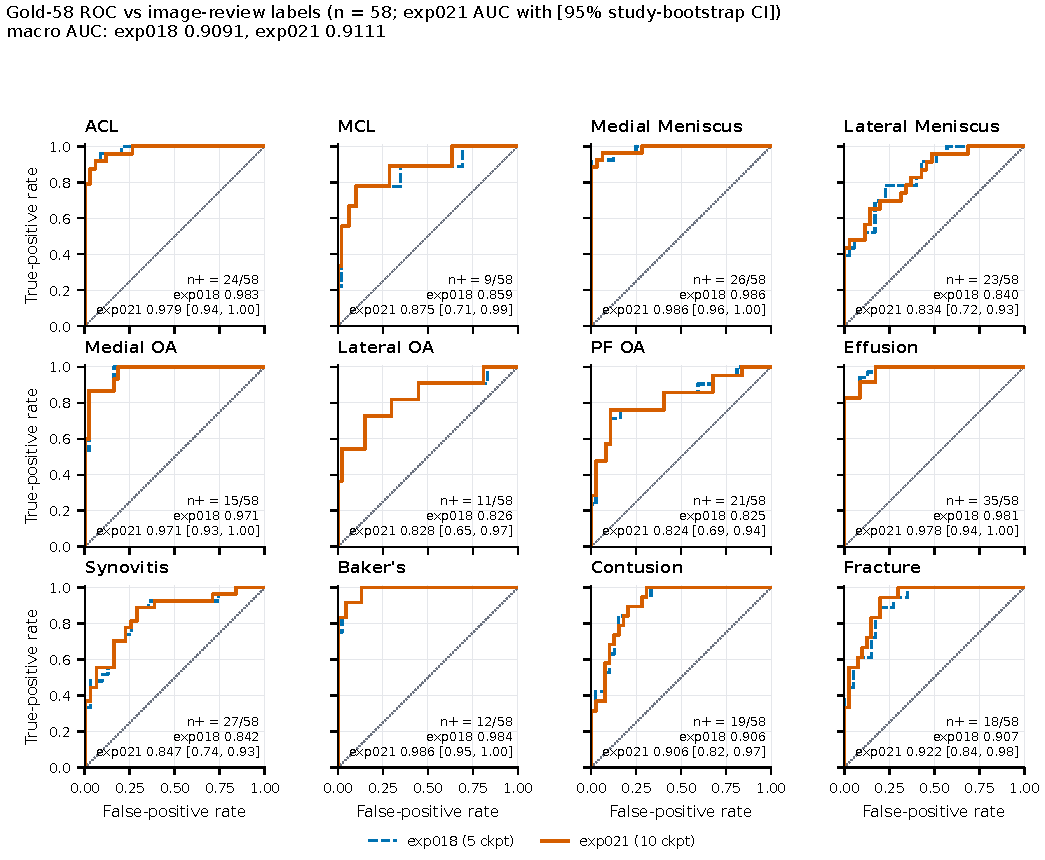
\includegraphics[width=0.93\textwidth]{roc_gold58_exp018_exp021.pdf}
\caption{Per-finding ROC curves on the 58 image-review studies (exp021 AUC with 95\% study-bootstrap interval).}
\label{fig:roc}
\end{figure*}
\begin{figure*}[t]
\centering
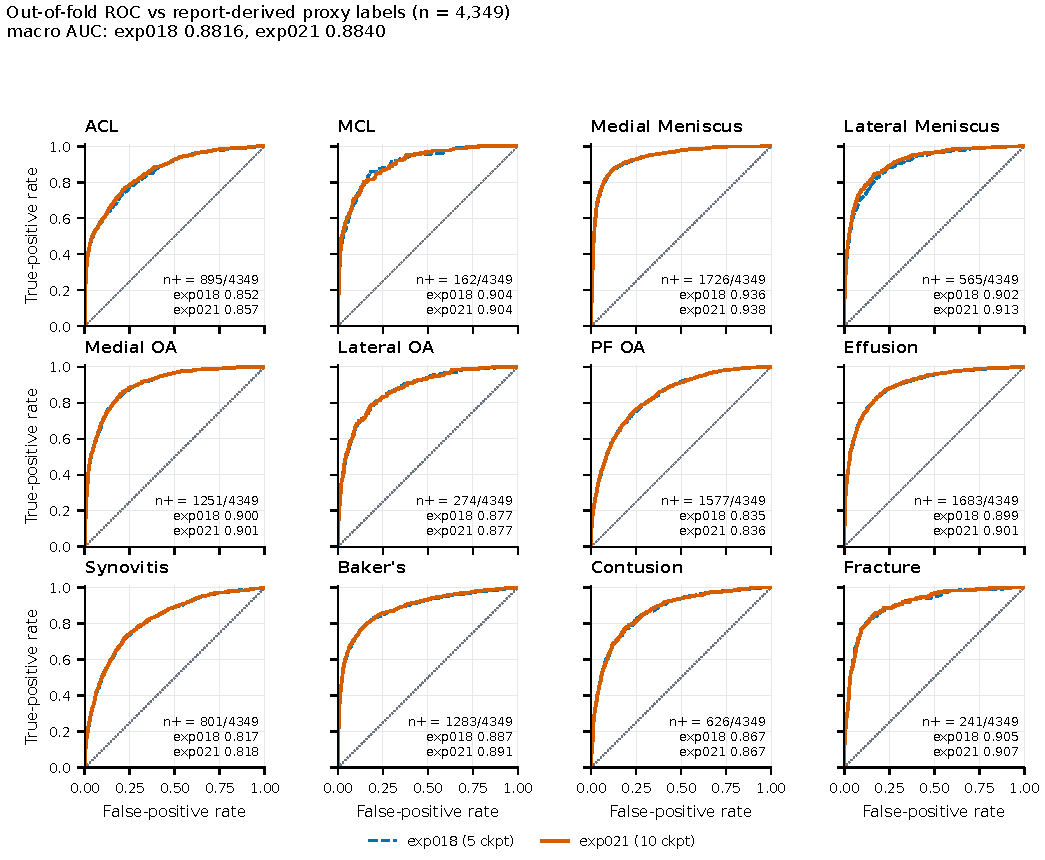
\includegraphics[width=0.93\textwidth]{roc_oof_exp018_exp021.pdf}
\caption{Out-of-fold ROC curves against report-derived labels ($n=4{,}349$).}
\label{fig:rocoof}
\end{figure*}
\fi

\begin{table}[t]
\caption{Efficiency track (maxAUC assumed 0.95; public AUC; lower is better).}
\label{tab:eff}
\centering\footnotesize
\begin{tabular}{@{}lccc@{}}
\toprule
Configuration & LB AUC & Time & Score \\
\midrule
Distilled DINOv2-S & 0.885 & $\sim$11.6 min$^{c}$ & $-1.945$ \\  % SRC: exp018_efficiency_table.md (projected runtime)
Window-MIL, 5 folds & 0.929 & $\sim$53 min & $-1.966$ \\             % SRC: computed: 0.929/(-0.45)+3180/32400
Window-MIL, 2 folds & 0.925 & $\sim$20.5 min & $\mathbf{-2.018}$ \\   % SRC: 2026-09-26 efficiency entries
\bottomrule
\end{tabular}\\[2pt]
{\footnotesize $^{c}$Projected, not measured.}
\end{table}
\begin{notes}
\begin{itemize}
\item \nt{Model-bound, not decode-bound: 5 folds take $\sim$4.5 s/study on one T4 ($\sim$53 min), so fold count is the lever;
2 folds run at the DICOM-decode floor.}  % SRC: 2026-09-26 "C" entries
\item \nt{Tested and not adopted: channels\_last ($-3.7\%$ time, predictions within $3\times10^{-4}$), 4th decode thread (no gain).}
\end{itemize}
\end{notes}

% ======================================================================================================
\section{Analysis}
\begin{figure*}[t]   % PLACEMENT: top of the page; slide variant has 3 rows (the 6-row version is attention_windows_gold58.pdf)
\centering
\includegraphics[width=0.8\textwidth]{attention_windows_gold58_slide.pdf}
\caption{Window-MIL attention (exp021, mean of 10 checkpoints) for three gold-positive studies: the four most-attended
windows and the attention over all windows. Studies were chosen by a fixed rule before any map was viewed (the most
confidently detected gold-positive study per finding); this is a best case, not a hit rate.}
\label{fig:attention}
\end{figure*}
\begin{notes}
\begin{itemize}
\item \nt{Attention view: ACL pools mostly from sagittal fat-suppressed slices, medial meniscus from coronal, Baker's cyst
from axial. Over all 58 gold studies: ACL 62\% of attention on sagittal FS (30\% if uniform), Baker's 45\% on axial (20\%
uniform), effusion 57\% sagittal FS.}  % SRC: docs/figures/attention_slot_mass_gold58.csv
\item \nt{Attention is broad: top-4 windows hold 22--48\% in the selected studies; a finding pools over about 16--40
effective windows (mean 52 windows per study).}  % SRC: same csv, column effective_windows
\item \nt{Caveat: this shows where the pooling draws from, not that it localizes the lesion; no radiologist reviewed the
windows; the two seed groups agree on window attention (per-finding Spearman 0.85--0.95).}  % SRC: csv, seed42_vs_seed43
\end{itemize}
\end{notes}
\ifextrafigs
\begin{figure}[t]
\centering
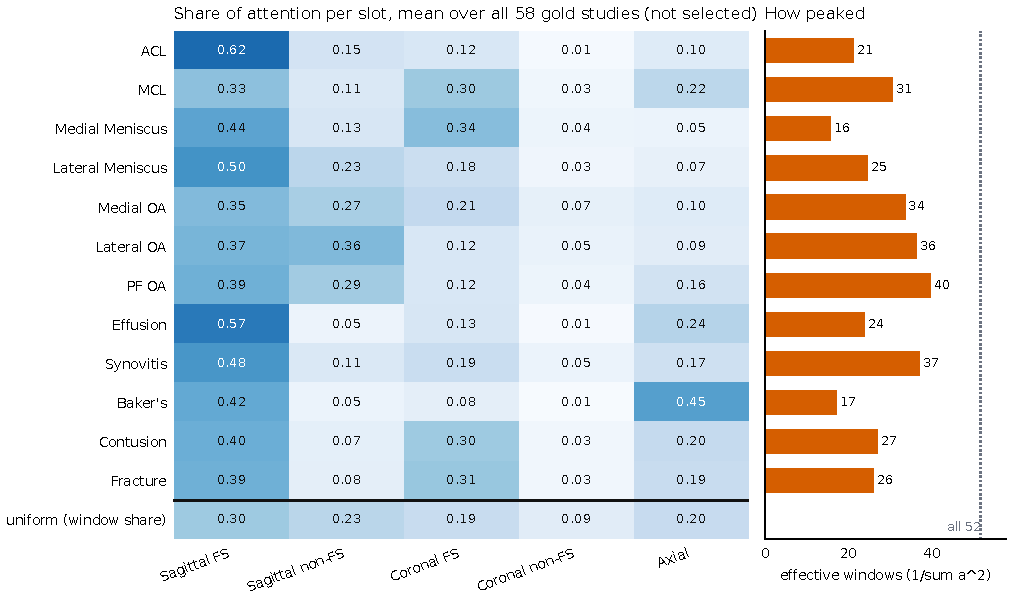
\includegraphics[width=\columnwidth]{attention_by_slot_gold58.pdf}
\caption{Share of attention per slot, all 58 gold studies (not selected), and how peaked the attention is.}
\label{fig:slotshare}
\end{figure}
\fi
\subsection{Validation lessons}
\begin{notes}
\begin{itemize}
\item \nt{OOF vs LB gaps: slot pipeline $\sim-0.030$ (0.8631 vs 0.893; first recorded as $-0.0186$ on the 3-member OOF,
corrected), exp008 $-0.014$ to $-0.020$, exp018 $-0.0474$. Reading: report-derived OOF is a conservative proxy; leakage would
push the other way.}  % SRC: 2026-10-01 correction; METHOD_WRITEUP s11
\item \nt{A runtime degradation ladder silently changed which model was scored: the 3-member notebook measures $\sim$59
s/study on T4 ($\sim$21~h), so it almost certainly ran exp005 alone (inferred, not confirmed). The efficiency notebook also
picked its fold count at run time (unknown). Log the chosen rung; measure on target hardware before trusting a score.}
  % SRC: 2026-09-27, 2026-10-01
\item \nt{Borrowed speed factors were off by 3.6$\times$ (CoAtNet) and $\sim$13$\times$ (DINOv2) between H100 and T4.}
\item \nt{Process lessons worth a sentence each: a ``root cause'' proven off-platform was not on the failing path; a timed join
silently wrote label priors; tests must assert on prediction content, not row counts.}  % SRC: METHOD_WRITEUP s9
\end{itemize}
\end{notes}

\section{Limitations}
\begin{notes}
\begin{itemize}
\item \nt{Gold-58 ($n=58$): 95\% CI about $\pm0.03$ on macro-AUC; differences below $\sim$0.02 cannot be resolved.}
\item \nt{Public leaderboard only; the final private rank is unknown until the competition closes (Oct 22).}
\item \nt{The 0.893 $\rightarrow$ 0.929 gain is not attributed to any single change; attention maps are unvalidated
by a clinician; the 0.893 attribution to exp005 is an inference.}
\item \nt{Label-engine calibration used the same 58 studies that report gold-58 AUC (leave-one-out for the labeler; the image
models never trained on them), so the labeler's own agreement numbers are optimistic.}
\item \nt{No external data; single-person project; Kaggle hardware only for inference.}
\end{itemize}
\end{notes}

\section{Conclusion}
\begin{notes}
\begin{itemize}
\item \nt{Three sentences: what worked (calibrated report labels; per-finding attention over windows; seed ensemble), what
did not (every slot-family lever; blends), and the methodological point (pre-registration, measured runtime, logged
fallbacks).}
\item \nt{Availability: code, weights and write-up to be released after Oct 22 (repository private until then). \todo{insert URL}}
\end{itemize}
\end{notes}

\section*{Acknowledgment}
\nt{Compute: university HPC cluster (H100) and Kaggle T4 notebooks. \todo{add course/instructor thanks}}

\bibliographystyle{IEEEtran}
\bibliography{refs}

\end{document}
"
\ifdefined\hidenotes\excludecomment{notes}\else\includecomment{notes}\fi
\graphicspath{{../figures/}}

\newcommand{\nt}[1]{\textcolor{gray}{\textit{#1}}}            % note-to-self (replace with prose)
\newcommand{\todo}[1]{\textcolor{red}{\textbf{[TODO: #1]}}}
\newif\ifextrafigs
\extrafigsfalse   % set \extrafigstrue to include the optional figures (OOF ROC, slot-share heat map)

\begin{document}

\title{Weak Supervision and Window-Level Attention for Knee-MRI Abnormality Detection:\\
Lessons from the RSNA 2026 Kaggle Challenge}   % working title

\author{\IEEEauthorblockN{Husnain Rasool}
\IEEEauthorblockA{\textit{[Department / course]} \\
\textit{[University]} \\
\textit{[email]}}}

\maketitle

\begin{abstract}
\nt{150--200 words. Must say: (1) 12 knee-MRI findings, macro ROC-AUC, only 58 of 4,407 training studies have
image-review labels, the rest have free-text reports (not available at test time); (2) a report-to-label engine
(two open LLMs, calibrated on the 58); (3) the DINOv2 slot model plateaued near 0.89 public AUC, a window-level
attention model reached 0.929 (the change bundled four things, none isolated); (4) the final model is a 10-checkpoint
ensemble of that model; a 2-fold version runs in about 20 minutes; (5) what was learned about validation and about
silent runtime fallbacks. Numbers: 0.893 $\rightarrow$ 0.929 public LB; OOF 0.8840; gold-58 0.9111.}
\end{abstract}

\begin{IEEEkeywords}
knee MRI, weak supervision, multiple-instance learning, attention, Kaggle, evaluation methodology
\end{IEEEkeywords}

% ======================================================================================================
\section{Introduction}
\begin{notes}
\begin{itemize}
\item \nt{The task: 12 binary findings per knee-MRI study (ACL, MCL, medial/lateral meniscus, three OA compartments,
effusion, synovitis, Baker's cyst, contusion, fracture); metric = macro-averaged ROC-AUC; Kaggle code competition
(GPU $\le$ 9 h, no internet), $\sim$1,300 hidden test studies.}  % SRC: CLAUDE.md s1
\item \nt{The difficulty is the supervision: 4,407 training studies, 58 with image-review labels, every study with a
radiology report in 12+ languages, no reports at test time; reports agree with image review only $\sim$82\%
(they over-call mild disease).}  % SRC: CLAUDE.md s2
\item \nt{Contributions, kept honest: (i) a report-to-label engine calibrated on 58 studies; (ii) a diagnosis of a
$\sim$0.89 plateau and a window-level attention model that scored 0.929 public (a bundled change, not an ablation);
(iii) a measurement-discipline thread: pre-registered bars, paired cluster bootstrap, runtime measured on the target
hardware, and the discovery that a runtime fallback silently changed which model was scored.}
\item \nt{State the scope limits early: public leaderboard only (private rank known Oct 22); gold set is $n=58$.}
\end{itemize}
\end{notes}

\section{Related Work}
\begin{notes}
\begin{itemize}
\item \nt{Public knee MRI benchmarks: MRNet~\cite{bien2018mrnet} (not used: licensing; no external data used).}
\item \nt{Report-derived labels: rule/LLM labelers for radiology reports, e.g. CheXpert~\cite{irvin2019chexpert}; here the
labeler is a rubric-conditioned open LLM calibrated on a tiny gold set.}
\item \nt{Noisy-student self-training~\cite{xie2020noisystudent} (used once: image-model out-of-fold predictions blended
back into the labels; a second round regressed).}
\item \nt{Attention-based multiple-instance learning~\cite{ilse2018attention}; backbones DINOv2~\cite{oquab2023dinov2} and
CoAtNet~\cite{dai2021coatnet} via timm~\cite{wightman2019timm}.}
\item \nt{The window-MIL design follows a public Kaggle kernel~\cite{dread2026kernel}; say so plainly (re-implemented, own
labels and folds, no third-party weights or labels).}
\item \nt{LLM tooling: Qwen2.5~\cite{qwen2025}, Llama~3~\cite{llama3}, vLLM~\cite{kwon2023vllm}.}
\item \todo{add the external published benchmark noted in EXPERIMENTS.md 2026-09-17 (``Qiu et al. 2024, Nat Commun''):
its title and DOI are not recorded in the repo.}
\end{itemize}
\end{notes}

\section{Data and Task}
\begin{notes}
\begin{itemize}
\item \nt{4,407 training studies, 24,371 series (mean 5.53 per study, range 3--14; sagittal 9,864, coronal 8,609,
axial 5,898); mixed DICOM transfer syntaxes (JPEG Lossless, JPEG 2000).}  % SRC: CLAUDE.md s3
\item \nt{Gold-58 positive rates (ACL .41 ... Effusion .60) show the label shift risk; test prevalence unknown.}
  % SRC: CLAUDE.md s3
\item \nt{Validation protocol: 5-fold GroupKFold over report-template clusters (3,681 clusters); gold-58 never trained
on; OOF macro-AUC against the report-derived proxy labels is the main selection signal, gold-58 a tripwire, public LB the
external check.}  % SRC: EXPERIMENTS.md 2026-09-20 results block (3,681 clusters)
\item \nt{Noise scale: paired cluster bootstrap SD of a solo macro-AUC $\approx 0.0041$, so 2 SD $=0.0082$ was the
pre-registered bar for ablations.}  % SRC: EXPERIMENTS.md ablation ledger conventions
\end{itemize}
\end{notes}

\section{Label Engine}
\begin{notes}
\begin{itemize}
\item \nt{Two open LLMs (Qwen2.5-72B-Instruct, Llama-3.3-70B) read each report against a per-finding rubric that encodes
the experts' severity thresholds (``on the fence'' = negative); structured output per finding.}
\item \nt{Per-label strategy (Qwen / Llama / blend) chosen by strict leave-one-out AUC on gold-58: macro LOO 0.823
(\texttt{labels\_v2\_final}); report-vs-gold agreement $\sim$82\%.}  % SRC: ledger LE3
\item \nt{Noisy-student round (\texttt{labels\_v3}): blend with an image model's out-of-fold predictions, weight per label
by LOO: chosen-blend LOO 0.904; accepted by a two-criterion test (OOF vs original labels 0.8631 vs 0.8489, gold-58
+0.0139). A second round (v4) regressed ($-0.012$ LOO) and was stopped.}  % SRC: ledger LE4, LE5
\item \nt{Effect of labels alone: +0.0142 OOF at fixed architecture (exp005 vs exp002).}  % SRC: ledger B
\end{itemize}
\end{notes}

\section{Image Models}
\begin{figure*}[t]   % PLACEMENT: top of the page where section V starts; full width
\centering
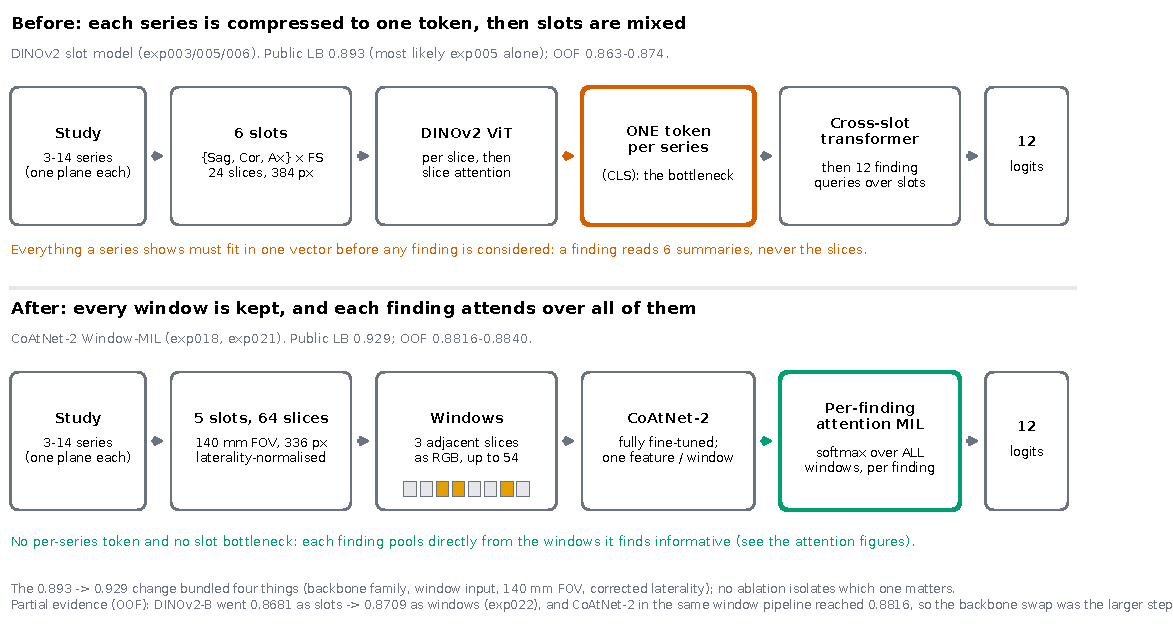
\includegraphics[width=0.97\textwidth]{formulation_before_after.pdf}
\caption{Series-token compression (DINOv2 slot model) versus per-finding window attention (CoAtNet-2 Window-MIL).
The 0.893 $\rightarrow$ 0.929 change bundled four things (backbone family, window input, 140~mm FOV, corrected
laterality); no ablation isolates which one matters.}
\label{fig:formulation}
\end{figure*}
\subsection{Slot model (first formulation)}
\begin{notes}
\begin{itemize}
\item \nt{DINOv2 ViT per slice (24 slices, 384 px) $\rightarrow$ slice-attention transformer $\rightarrow$ one CLS token per
series $\rightarrow$ 6 slots \{sag, cor, ax\}$\times$\{fluid-sensitive or not\} $\rightarrow$ cross-slot transformer $\rightarrow$
12 per-finding queries.}  % SRC: README.md "How it works" 3; src/rsna_knee/model.py
\item \nt{OOF: ViT-S 0.8631 (v3 labels), ViT-B 0.8681, 3-member ensemble 0.8744.}  % SRC: ledger B
\end{itemize}
\end{notes}
\subsection{Window-MIL (final formulation)}
\begin{notes}
\begin{itemize}
\item \nt{140~mm FOV at 336 px, 64 slices over five slots (18/14/12/8/12), laterality-normalized; windows of 3 adjacent
slices as RGB (at most 54 per study); fully fine-tuned CoAtNet-2; per-finding attention over all windows.}
  % SRC: README.md "How it works" 2; src/rsna_knee/wmil.py
\item \nt{Laterality: coronal/axial mirrored for right knees, sagittal slice order reversed; side from validated table,
then DICOM tag, then an image-centre geometry rule (99.4\% of the 1,491 studies previously un-normalized; 99.0--99.1\%
agreement).}  % SRC: METHOD_WRITEUP s5a; exp018_cache_audit.md
\item \nt{Training: top-3 epoch weight averaging; labels v3; pre-registered fold-0 kill rule (gold-58 $<$ 0.880).}
\item \nt{Final main model: exp021 = 10 checkpoints (seed 42 and 43, five folds each, probability mean). Efficiency model:
exp018 folds 0--1 only.}
\end{itemize}
\end{notes}
\subsection{Evaluation and efficiency track}
\begin{notes}
\begin{itemize}
\item \nt{Efficiency score $=\text{AUC}/(0.5-\max\text{AUC}) + t/32400$ (minimised); $\max\text{AUC}=0.95$ is an
assumption here.}  % SRC: CLAUDE.md s4
\item \nt{Inference in fp16 (never bf16 on T4); two T4 GPUs; runtimes measured on Kaggle's own machine.}
\end{itemize}
\end{notes}

% ======================================================================================================
\section{Results}
\begin{table}[t]   % PLACEMENT: right after the section heading
\caption{Main results. OOF is scored against report-derived labels; gold-58 against image-review labels (fold-ensembled);
LB is the public leaderboard. Runtimes are measured on Kaggle's 2$\times$T4 for $\sim$1,300 studies.}
\label{tab:main}
\centering\footnotesize
\begin{tabular}{@{}p{2.55cm}cccc@{}}
\toprule
Model & OOF & Gold-58 & LB & Time \\
\midrule
DINOv2 slot pipeline$^{a}$ & 0.8631 & 0.8903 & 0.893 & --- \\  % SRC: 2026-10-01 re-gate (exp005 0.8631/0.8903); 0.893 LB
Distilled DINOv2-S$^{b}$ & 0.8708 & 0.888 & 0.885 & --- \\       % SRC: ledger B (exp008 0.8708/0.8882); METHOD_WRITEUP s11 (0.885)
Window-MIL, 5 folds (exp018) & 0.8816 & 0.9091 & 0.929 & $\sim$53 min \\   % SRC: 2026-09-21 result; 2026-09-26 profile
Window-MIL, 10 ckpt (exp021) & \textbf{0.8840} & \textbf{0.9111} & \textbf{0.929} & $\sim$100 min \\ % SRC: 2026-09-25
Window-MIL, 2 folds & n/a & 0.9078 & 0.925 & $\sim$20.5 min \\     % SRC: README.md results; 2026-09-26 probes #5/#6
\bottomrule
\end{tabular}\\[2pt]
{\footnotesize $^{a}$Most likely exp005 alone after the notebook's runtime fallback (inferred; the 3-member ensemble
measures $\sim$21~h on T4). $^{b}$Fold count chosen at run time; the scored count is unknown.}
\end{table}
\begin{notes}
\begin{itemize}
\item \nt{Say the 0.893 attribution here (see Limitations): the notebook chooses its configuration from a time budget.}
\item \nt{exp021 over exp018: OOF +0.0024, 95\% paired CI [+0.0014, +0.0033]; gold-58 +0.0021 (CI spans zero).}
  % SRC: EXPERIMENTS.md 2026-09-25
\item \nt{Leaderboard beat OOF every time: about +0.030 (slot pipeline, corrected), +0.047 (exp018); OOF is scored against
noisy report labels.}  % SRC: 2026-10-01 correction; 2026-09-22
\end{itemize}
\end{notes}

\begin{figure*}[t]   % PLACEMENT: top of the next page
\centering
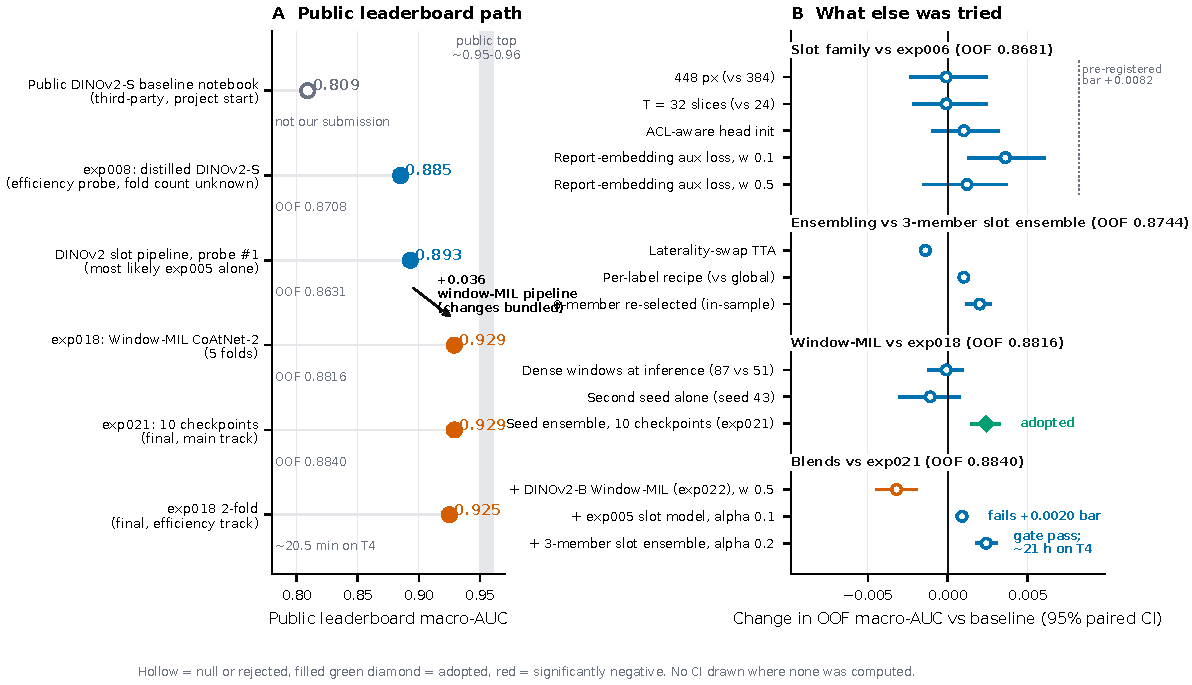
\includegraphics[width=0.93\textwidth]{ablation_path_and_nulls.pdf}
\caption{(A) Public leaderboard path (the 0.809 baseline is a third-party notebook, not a submission). (B) Every tested
change as a paired OOF delta with its 95\% cluster-bootstrap interval, grouped by baseline.}
\label{fig:ablation}
\end{figure*}

\begin{table*}[t]   % PLACEMENT: after Fig. 2; filled from docs/EXPERIMENTS.md (section per row in the SRC comments)
\caption{Ablation ledger. $\Delta$ is OOF macro-AUC against the stated baseline; intervals are paired cluster bootstrap
over 3,681 report clusters unless noted. ``Bar'' is the pre-registered $+0.0082$ for the slot family.}
\label{tab:ablation}
\centering\footnotesize
\begin{tabular}{@{}llccl@{}}
\toprule
Change & Baseline (OOF) & $\Delta$ OOF & 95\% CI & Verdict \\
\midrule
448 px (vs 384) & exp006 (0.8681) & $-0.0001$ & [$-0.0024$, $+0.0025$] & null \\          % SRC: ledger C, exp015
$T=32$ slices (vs 24) & exp006 & $-0.0001$ & [$-0.0022$, $+0.0025$] & null \\              % SRC: ledger C, exp010
ACL-aware head init & exp006 & $+0.0010$ & [$-0.0010$, $+0.0032$] & null (MCL $-0.0122$) \\ % SRC: 2026-09-20 block, exp012
Report-embedding aux loss, $w=0.1$ & exp006 & $+0.0036$ & [$+0.0012$, $+0.0061$] & below bar \\ % SRC: ledger C, exp016a
Report-embedding aux loss, $w=0.5$ & exp006 & $+0.0012$ & [$-0.0016$, $+0.0037$] & null \\ % SRC: ledger C, exp016b
Laterality-swap TTA & 3-member (0.8744) & $-0.0014$ & --- & rejected \\               % SRC: ledger D
Per-label ensemble recipe & 3-member & $+0.0010$ & --- & below $0.002$ bar \\          % SRC: ledger D
6-member re-selected ensemble & 3-member & $+0.0020$ & [$+0.0011$, $+0.0027$] & in-sample; $2.9\times$ cost \\ % SRC: ledger D
Dense windows at inference (87 vs 51) & exp018 (0.8816) & $-0.0001$ & [$-0.0013$, $+0.0010$] & null \\ % SRC: 2026-09-26 dense
Second seed alone (seed 43) & exp018 & $-0.0011$ & [$-0.0031$, $+0.0008$] & null \\       % SRC: 2026-09-25 exp021
\textbf{10-checkpoint seed ensemble} & exp018 & $+0.0024$ & [$+0.0014$, $+0.0033$] & \textbf{adopted} \\ % SRC: 2026-09-25
DINOv2-B inside the window pipeline (solo) & exp018 & $-0.0107$ & --- & worse (0.8709) \\ % SRC: 2026-09-26 exp022; delta = 0.8709-0.8816
EMA, decay 0.999 (fold 0, gold-58) & top-3 average & $-0.0009$ & --- & null \\         % SRC: 2026-09-24 exp020 (fold-0 gold-58, not OOF)
+ DINOv2-B window model, $w=0.5$ & exp021 (0.8840) & $-0.0032$ & [$-0.0045$, $-0.0019$] & gate fail \\ % SRC: 2026-09-26 exp022
+ 3-member slot ensemble, $\alpha=0.2$ & exp021 & $+0.0024$ & [$+0.0017$, $+0.0031$] & gate pass; $\sim$21 h on T4 \\ % SRC: 2026-09-26 gate
+ exp005, $\alpha=0.1$ & exp021 & $+0.0009$ & [$+0.0005$, $+0.0012$] & below $+0.0020$ bar \\ % SRC: 2026-10-01 re-gate
\bottomrule
\end{tabular}
\end{table*}
\begin{notes}
\begin{itemize}
\item \nt{Write the null-result paragraph: six pre-registered slot-family changes inside noise; ViT-S$\to$ViT-B
($+0.005$), v3 labels ($+0.014$) and ensembling ($+0.006$) were the only early gains; the plateau was a property of
the model family.}  % SRC: ledger "Reading the whole record"
\item \nt{Other rejected items worth one clause: DINOv3-S ($-0.0252$), ConvNeXt-V2 (redundant, corr 0.93), 3D ResNet
(killed), CoAtNet-3 (no result: no pretrained checkpoint at the intended size, then a 32-bit indexing overflow).}
  % SRC: ledger B; 2026-09-24
\item \nt{The blend: the 3-member arm passes an offline gate but cannot run in time on T4; the single-model arm fails the
bar; modeling closed.}  % SRC: 2026-09-27, 2026-10-01
\end{itemize}
\end{notes}

\begin{table}[t]   % PLACEMENT: column width; numbers generated by scripts/report_tables.py
\caption{Per-label AUC. OOF: 4,349 studies against report-derived labels; gold-58: against image review.}
\label{tab:perlabel}
\centering\footnotesize
\begin{tabular}{@{}lcccc@{}}
\toprule
 & \multicolumn{2}{c}{OOF} & \multicolumn{2}{c}{Gold-58} \\
\cmidrule(lr){2-3}\cmidrule(lr){4-5}
Finding & exp018 & exp021 & exp018 & exp021 \\
\midrule
ACL & 0.852 & 0.857 & 0.983 & 0.979 \\
MCL & 0.904 & 0.904 & 0.859 & 0.875 \\
Medial Meniscus & 0.936 & 0.938 & 0.986 & 0.986 \\
Lateral Meniscus & 0.902 & 0.913 & 0.840 & 0.834 \\
Medial OA & 0.900 & 0.901 & 0.971 & 0.971 \\
Lateral OA & 0.877 & 0.877 & 0.826 & 0.828 \\
PF OA & 0.835 & 0.836 & 0.825 & 0.824 \\
Effusion & 0.899 & 0.901 & 0.981 & 0.978 \\
Synovitis & 0.817 & 0.818 & 0.842 & 0.847 \\
Baker's & 0.887 & 0.891 & 0.984 & 0.986 \\
Contusion & 0.867 & 0.867 & 0.906 & 0.906 \\
Fracture & 0.905 & 0.907 & 0.907 & 0.922 \\
\midrule
Macro & 0.8816 & 0.8840 & 0.9091 & 0.9111
 \\
\bottomrule
\end{tabular}
\end{table}
\begin{notes}
\begin{itemize}
\item \nt{ACL: lowest-ish on OOF (0.857) but 0.979 on gold-58, so the OOF deficit is proxy-label noise.}
  % SRC: table above; EXPERIMENTS.md 2026-09-18 ACL conclusion
\item \nt{Weakest on gold-58: PF OA 0.824, lateral OA 0.828, lateral meniscus 0.834 ($n=58$: wide intervals).}
\end{itemize}
\end{notes}

\ifextrafigs   % optional: ~0.6 page; the per-label table carries the same numbers
\begin{figure*}[t]
\centering
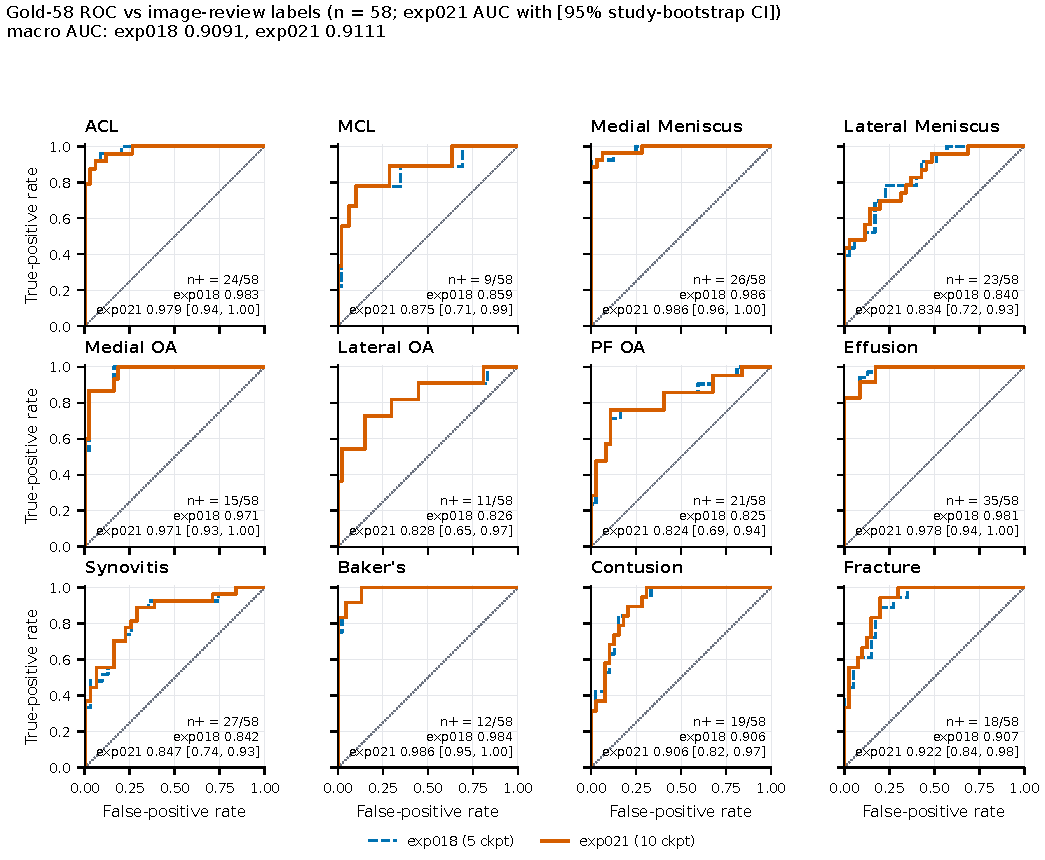
\includegraphics[width=0.93\textwidth]{roc_gold58_exp018_exp021.pdf}
\caption{Per-finding ROC curves on the 58 image-review studies (exp021 AUC with 95\% study-bootstrap interval).}
\label{fig:roc}
\end{figure*}
\begin{figure*}[t]
\centering
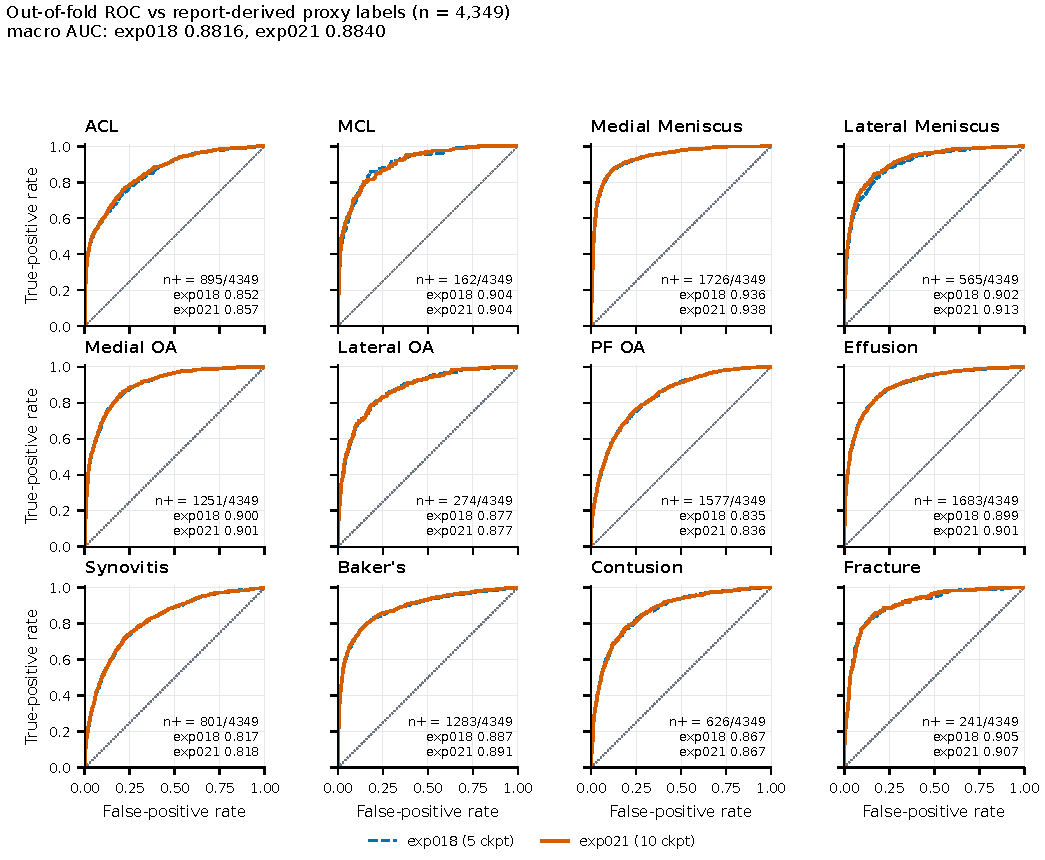
\includegraphics[width=0.93\textwidth]{roc_oof_exp018_exp021.pdf}
\caption{Out-of-fold ROC curves against report-derived labels ($n=4{,}349$).}
\label{fig:rocoof}
\end{figure*}
\fi

\begin{table}[t]
\caption{Efficiency track (maxAUC assumed 0.95; public AUC; lower is better).}
\label{tab:eff}
\centering\footnotesize
\begin{tabular}{@{}lccc@{}}
\toprule
Configuration & LB AUC & Time & Score \\
\midrule
Distilled DINOv2-S & 0.885 & $\sim$11.6 min$^{c}$ & $-1.945$ \\  % SRC: exp018_efficiency_table.md (projected runtime)
Window-MIL, 5 folds & 0.929 & $\sim$53 min & $-1.966$ \\             % SRC: computed: 0.929/(-0.45)+3180/32400
Window-MIL, 2 folds & 0.925 & $\sim$20.5 min & $\mathbf{-2.018}$ \\   % SRC: 2026-09-26 efficiency entries
\bottomrule
\end{tabular}\\[2pt]
{\footnotesize $^{c}$Projected, not measured.}
\end{table}
\begin{notes}
\begin{itemize}
\item \nt{Model-bound, not decode-bound: 5 folds take $\sim$4.5 s/study on one T4 ($\sim$53 min), so fold count is the lever;
2 folds run at the DICOM-decode floor.}  % SRC: 2026-09-26 "C" entries
\item \nt{Tested and not adopted: channels\_last ($-3.7\%$ time, predictions within $3\times10^{-4}$), 4th decode thread (no gain).}
\end{itemize}
\end{notes}

% ======================================================================================================
\section{Analysis}
\begin{figure*}[t]   % PLACEMENT: top of the page; slide variant has 3 rows (the 6-row version is attention_windows_gold58.pdf)
\centering
\includegraphics[width=0.8\textwidth]{attention_windows_gold58_slide.pdf}
\caption{Window-MIL attention (exp021, mean of 10 checkpoints) for three gold-positive studies: the four most-attended
windows and the attention over all windows. Studies were chosen by a fixed rule before any map was viewed (the most
confidently detected gold-positive study per finding); this is a best case, not a hit rate.}
\label{fig:attention}
\end{figure*}
\begin{notes}
\begin{itemize}
\item \nt{Attention view: ACL pools mostly from sagittal fat-suppressed slices, medial meniscus from coronal, Baker's cyst
from axial. Over all 58 gold studies: ACL 62\% of attention on sagittal FS (30\% if uniform), Baker's 45\% on axial (20\%
uniform), effusion 57\% sagittal FS.}  % SRC: docs/figures/attention_slot_mass_gold58.csv
\item \nt{Attention is broad: top-4 windows hold 22--48\% in the selected studies; a finding pools over about 16--40
effective windows (mean 52 windows per study).}  % SRC: same csv, column effective_windows
\item \nt{Caveat: this shows where the pooling draws from, not that it localizes the lesion; no radiologist reviewed the
windows; the two seed groups agree on window attention (per-finding Spearman 0.85--0.95).}  % SRC: csv, seed42_vs_seed43
\end{itemize}
\end{notes}
\ifextrafigs
\begin{figure}[t]
\centering
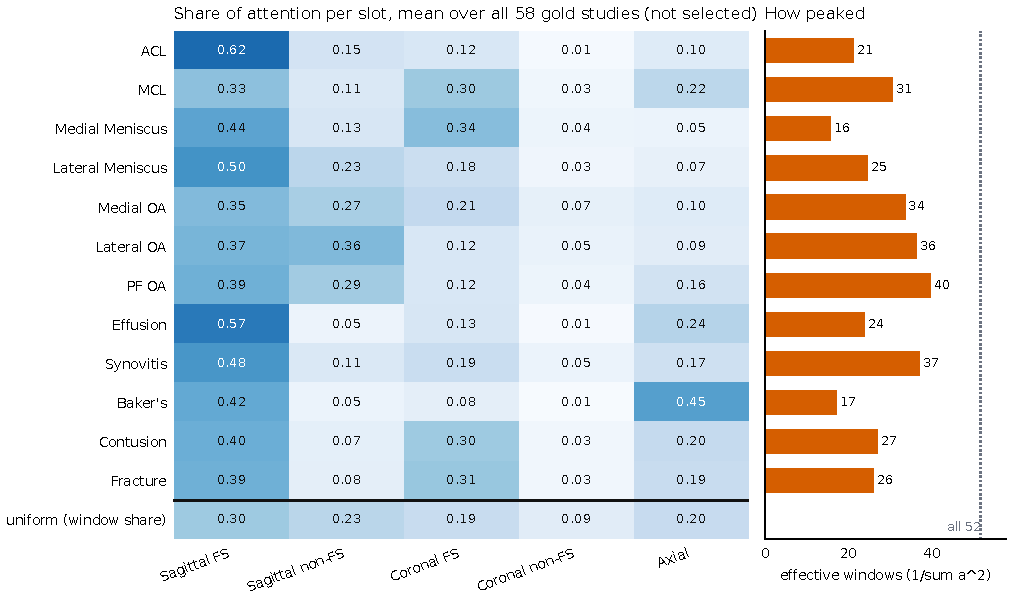
\includegraphics[width=\columnwidth]{attention_by_slot_gold58.pdf}
\caption{Share of attention per slot, all 58 gold studies (not selected), and how peaked the attention is.}
\label{fig:slotshare}
\end{figure}
\fi
\subsection{Validation lessons}
\begin{notes}
\begin{itemize}
\item \nt{OOF vs LB gaps: slot pipeline $\sim-0.030$ (0.8631 vs 0.893; first recorded as $-0.0186$ on the 3-member OOF,
corrected), exp008 $-0.014$ to $-0.020$, exp018 $-0.0474$. Reading: report-derived OOF is a conservative proxy; leakage would
push the other way.}  % SRC: 2026-10-01 correction; METHOD_WRITEUP s11
\item \nt{A runtime degradation ladder silently changed which model was scored: the 3-member notebook measures $\sim$59
s/study on T4 ($\sim$21~h), so it almost certainly ran exp005 alone (inferred, not confirmed). The efficiency notebook also
picked its fold count at run time (unknown). Log the chosen rung; measure on target hardware before trusting a score.}
  % SRC: 2026-09-27, 2026-10-01
\item \nt{Borrowed speed factors were off by 3.6$\times$ (CoAtNet) and $\sim$13$\times$ (DINOv2) between H100 and T4.}
\item \nt{Process lessons worth a sentence each: a ``root cause'' proven off-platform was not on the failing path; a timed join
silently wrote label priors; tests must assert on prediction content, not row counts.}  % SRC: METHOD_WRITEUP s9
\end{itemize}
\end{notes}

\section{Limitations}
\begin{notes}
\begin{itemize}
\item \nt{Gold-58 ($n=58$): 95\% CI about $\pm0.03$ on macro-AUC; differences below $\sim$0.02 cannot be resolved.}
\item \nt{Public leaderboard only; the final private rank is unknown until the competition closes (Oct 22).}
\item \nt{The 0.893 $\rightarrow$ 0.929 gain is not attributed to any single change; attention maps are unvalidated
by a clinician; the 0.893 attribution to exp005 is an inference.}
\item \nt{Label-engine calibration used the same 58 studies that report gold-58 AUC (leave-one-out for the labeler; the image
models never trained on them), so the labeler's own agreement numbers are optimistic.}
\item \nt{No external data; single-person project; Kaggle hardware only for inference.}
\end{itemize}
\end{notes}

\section{Conclusion}
\begin{notes}
\begin{itemize}
\item \nt{Three sentences: what worked (calibrated report labels; per-finding attention over windows; seed ensemble), what
did not (every slot-family lever; blends), and the methodological point (pre-registration, measured runtime, logged
fallbacks).}
\item \nt{Availability: code, weights and write-up to be released after Oct 22 (repository private until then). \todo{insert URL}}
\end{itemize}
\end{notes}

\section*{Acknowledgment}
\nt{Compute: university HPC cluster (H100) and Kaggle T4 notebooks. \todo{add course/instructor thanks}}

\bibliographystyle{IEEEtran}
\bibliography{refs}

\end{document}
"
\ifdefined\hidenotes\excludecomment{notes}\else\includecomment{notes}\fi
\graphicspath{{../figures/}}

\newcommand{\nt}[1]{\textcolor{gray}{\textit{#1}}}            % note-to-self (replace with prose)
\newcommand{\todo}[1]{\textcolor{red}{\textbf{[TODO: #1]}}}
\newif\ifextrafigs
\extrafigsfalse   % set \extrafigstrue to include the optional figures (OOF ROC, slot-share heat map)

\begin{document}

\title{Weak Supervision and Window-Level Attention for Knee-MRI Abnormality Detection:\\
Lessons from the RSNA 2026 Kaggle Challenge}   % working title

\author{\IEEEauthorblockN{Husnain Rasool}
\IEEEauthorblockA{\textit{[Department / course]} \\
\textit{[University]} \\
\textit{[email]}}}

\maketitle

\begin{abstract}
\nt{150--200 words. Must say: (1) 12 knee-MRI findings, macro ROC-AUC, only 58 of 4,407 training studies have
image-review labels, the rest have free-text reports (not available at test time); (2) a report-to-label engine
(two open LLMs, calibrated on the 58); (3) the DINOv2 slot model plateaued near 0.89 public AUC, a window-level
attention model reached 0.929 (the change bundled four things, none isolated); (4) the final model is a 10-checkpoint
ensemble of that model; a 2-fold version runs in about 20 minutes; (5) what was learned about validation and about
silent runtime fallbacks. Numbers: 0.893 $\rightarrow$ 0.929 public LB; OOF 0.8840; gold-58 0.9111.}
\end{abstract}

\begin{IEEEkeywords}
knee MRI, weak supervision, multiple-instance learning, attention, Kaggle, evaluation methodology
\end{IEEEkeywords}

% ======================================================================================================
\section{Introduction}
\begin{notes}
\begin{itemize}
\item \nt{The task: 12 binary findings per knee-MRI study (ACL, MCL, medial/lateral meniscus, three OA compartments,
effusion, synovitis, Baker's cyst, contusion, fracture); metric = macro-averaged ROC-AUC; Kaggle code competition
(GPU $\le$ 9 h, no internet), $\sim$1,300 hidden test studies.}  % SRC: CLAUDE.md s1
\item \nt{The difficulty is the supervision: 4,407 training studies, 58 with image-review labels, every study with a
radiology report in 12+ languages, no reports at test time; reports agree with image review only $\sim$82\%
(they over-call mild disease).}  % SRC: CLAUDE.md s2
\item \nt{Contributions, kept honest: (i) a report-to-label engine calibrated on 58 studies; (ii) a diagnosis of a
$\sim$0.89 plateau and a window-level attention model that scored 0.929 public (a bundled change, not an ablation);
(iii) a measurement-discipline thread: pre-registered bars, paired cluster bootstrap, runtime measured on the target
hardware, and the discovery that a runtime fallback silently changed which model was scored.}
\item \nt{State the scope limits early: public leaderboard only (private rank known Oct 22); gold set is $n=58$.}
\end{itemize}
\end{notes}

\section{Related Work}
\begin{notes}
\begin{itemize}
\item \nt{Public knee MRI benchmarks: MRNet~\cite{bien2018mrnet} (not used: licensing; no external data used).}
\item \nt{Report-derived labels: rule/LLM labelers for radiology reports, e.g. CheXpert~\cite{irvin2019chexpert}; here the
labeler is a rubric-conditioned open LLM calibrated on a tiny gold set.}
\item \nt{Noisy-student self-training~\cite{xie2020noisystudent} (used once: image-model out-of-fold predictions blended
back into the labels; a second round regressed).}
\item \nt{Attention-based multiple-instance learning~\cite{ilse2018attention}; backbones DINOv2~\cite{oquab2023dinov2} and
CoAtNet~\cite{dai2021coatnet} via timm~\cite{wightman2019timm}.}
\item \nt{The window-MIL design follows a public Kaggle kernel~\cite{dread2026kernel}; say so plainly (re-implemented, own
labels and folds, no third-party weights or labels).}
\item \nt{LLM tooling: Qwen2.5~\cite{qwen2025}, Llama~3~\cite{llama3}, vLLM~\cite{kwon2023vllm}.}
\item \todo{add the external published benchmark noted in EXPERIMENTS.md 2026-09-17 (``Qiu et al. 2024, Nat Commun''):
its title and DOI are not recorded in the repo.}
\end{itemize}
\end{notes}

\section{Data and Task}
\begin{notes}
\begin{itemize}
\item \nt{4,407 training studies, 24,371 series (mean 5.53 per study, range 3--14; sagittal 9,864, coronal 8,609,
axial 5,898); mixed DICOM transfer syntaxes (JPEG Lossless, JPEG 2000).}  % SRC: CLAUDE.md s3
\item \nt{Gold-58 positive rates (ACL .41 ... Effusion .60) show the label shift risk; test prevalence unknown.}
  % SRC: CLAUDE.md s3
\item \nt{Validation protocol: 5-fold GroupKFold over report-template clusters (3,681 clusters); gold-58 never trained
on; OOF macro-AUC against the report-derived proxy labels is the main selection signal, gold-58 a tripwire, public LB the
external check.}  % SRC: EXPERIMENTS.md 2026-09-20 results block (3,681 clusters)
\item \nt{Noise scale: paired cluster bootstrap SD of a solo macro-AUC $\approx 0.0041$, so 2 SD $=0.0082$ was the
pre-registered bar for ablations.}  % SRC: EXPERIMENTS.md ablation ledger conventions
\end{itemize}
\end{notes}

\section{Label Engine}
\begin{notes}
\begin{itemize}
\item \nt{Two open LLMs (Qwen2.5-72B-Instruct, Llama-3.3-70B) read each report against a per-finding rubric that encodes
the experts' severity thresholds (``on the fence'' = negative); structured output per finding.}
\item \nt{Per-label strategy (Qwen / Llama / blend) chosen by strict leave-one-out AUC on gold-58: macro LOO 0.823
(\texttt{labels\_v2\_final}); report-vs-gold agreement $\sim$82\%.}  % SRC: ledger LE3
\item \nt{Noisy-student round (\texttt{labels\_v3}): blend with an image model's out-of-fold predictions, weight per label
by LOO: chosen-blend LOO 0.904; accepted by a two-criterion test (OOF vs original labels 0.8631 vs 0.8489, gold-58
+0.0139). A second round (v4) regressed ($-0.012$ LOO) and was stopped.}  % SRC: ledger LE4, LE5
\item \nt{Effect of labels alone: +0.0142 OOF at fixed architecture (exp005 vs exp002).}  % SRC: ledger B
\end{itemize}
\end{notes}

\section{Image Models}
\begin{figure*}[t]   % PLACEMENT: top of the page where section V starts; full width
\centering
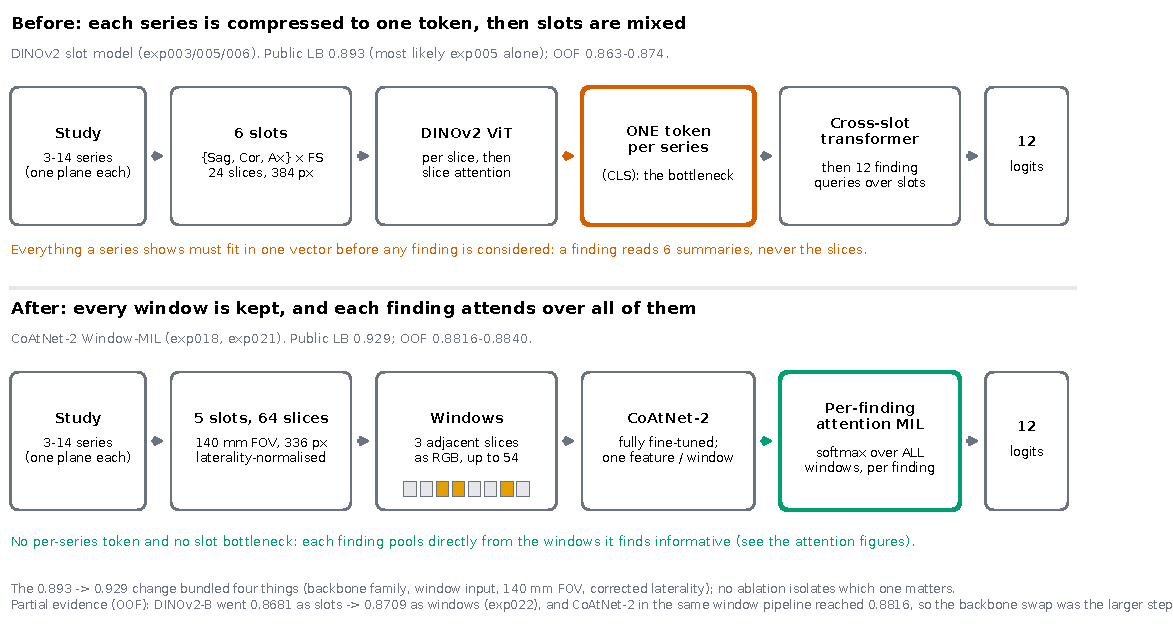
\includegraphics[width=0.97\textwidth]{formulation_before_after.pdf}
\caption{Series-token compression (DINOv2 slot model) versus per-finding window attention (CoAtNet-2 Window-MIL).
The 0.893 $\rightarrow$ 0.929 change bundled four things (backbone family, window input, 140~mm FOV, corrected
laterality); no ablation isolates which one matters.}
\label{fig:formulation}
\end{figure*}
\subsection{Slot model (first formulation)}
\begin{notes}
\begin{itemize}
\item \nt{DINOv2 ViT per slice (24 slices, 384 px) $\rightarrow$ slice-attention transformer $\rightarrow$ one CLS token per
series $\rightarrow$ 6 slots \{sag, cor, ax\}$\times$\{fluid-sensitive or not\} $\rightarrow$ cross-slot transformer $\rightarrow$
12 per-finding queries.}  % SRC: README.md "How it works" 3; src/rsna_knee/model.py
\item \nt{OOF: ViT-S 0.8631 (v3 labels), ViT-B 0.8681, 3-member ensemble 0.8744.}  % SRC: ledger B
\end{itemize}
\end{notes}
\subsection{Window-MIL (final formulation)}
\begin{notes}
\begin{itemize}
\item \nt{140~mm FOV at 336 px, 64 slices over five slots (18/14/12/8/12), laterality-normalized; windows of 3 adjacent
slices as RGB (at most 54 per study); fully fine-tuned CoAtNet-2; per-finding attention over all windows.}
  % SRC: README.md "How it works" 2; src/rsna_knee/wmil.py
\item \nt{Laterality: coronal/axial mirrored for right knees, sagittal slice order reversed; side from validated table,
then DICOM tag, then an image-centre geometry rule (99.4\% of the 1,491 studies previously un-normalized; 99.0--99.1\%
agreement).}  % SRC: METHOD_WRITEUP s5a; exp018_cache_audit.md
\item \nt{Training: top-3 epoch weight averaging; labels v3; pre-registered fold-0 kill rule (gold-58 $<$ 0.880).}
\item \nt{Final main model: exp021 = 10 checkpoints (seed 42 and 43, five folds each, probability mean). Efficiency model:
exp018 folds 0--1 only.}
\end{itemize}
\end{notes}
\subsection{Evaluation and efficiency track}
\begin{notes}
\begin{itemize}
\item \nt{Efficiency score $=\text{AUC}/(0.5-\max\text{AUC}) + t/32400$ (minimised); $\max\text{AUC}=0.95$ is an
assumption here.}  % SRC: CLAUDE.md s4
\item \nt{Inference in fp16 (never bf16 on T4); two T4 GPUs; runtimes measured on Kaggle's own machine.}
\end{itemize}
\end{notes}

% ======================================================================================================
\section{Results}
\begin{table}[t]   % PLACEMENT: right after the section heading
\caption{Main results. OOF is scored against report-derived labels; gold-58 against image-review labels (fold-ensembled);
LB is the public leaderboard. Runtimes are measured on Kaggle's 2$\times$T4 for $\sim$1,300 studies.}
\label{tab:main}
\centering\footnotesize
\begin{tabular}{@{}p{2.55cm}cccc@{}}
\toprule
Model & OOF & Gold-58 & LB & Time \\
\midrule
DINOv2 slot pipeline$^{a}$ & 0.8631 & 0.8903 & 0.893 & --- \\  % SRC: 2026-10-01 re-gate (exp005 0.8631/0.8903); 0.893 LB
Distilled DINOv2-S$^{b}$ & 0.8708 & 0.888 & 0.885 & --- \\       % SRC: ledger B (exp008 0.8708/0.8882); METHOD_WRITEUP s11 (0.885)
Window-MIL, 5 folds (exp018) & 0.8816 & 0.9091 & 0.929 & $\sim$53 min \\   % SRC: 2026-09-21 result; 2026-09-26 profile
Window-MIL, 10 ckpt (exp021) & \textbf{0.8840} & \textbf{0.9111} & \textbf{0.929} & $\sim$100 min \\ % SRC: 2026-09-25
Window-MIL, 2 folds & n/a & 0.9078 & 0.925 & $\sim$20.5 min \\     % SRC: README.md results; 2026-09-26 probes #5/#6
\bottomrule
\end{tabular}\\[2pt]
{\footnotesize $^{a}$Most likely exp005 alone after the notebook's runtime fallback (inferred; the 3-member ensemble
measures $\sim$21~h on T4). $^{b}$Fold count chosen at run time; the scored count is unknown.}
\end{table}
\begin{notes}
\begin{itemize}
\item \nt{Say the 0.893 attribution here (see Limitations): the notebook chooses its configuration from a time budget.}
\item \nt{exp021 over exp018: OOF +0.0024, 95\% paired CI [+0.0014, +0.0033]; gold-58 +0.0021 (CI spans zero).}
  % SRC: EXPERIMENTS.md 2026-09-25
\item \nt{Leaderboard beat OOF every time: about +0.030 (slot pipeline, corrected), +0.047 (exp018); OOF is scored against
noisy report labels.}  % SRC: 2026-10-01 correction; 2026-09-22
\end{itemize}
\end{notes}

\begin{figure*}[t]   % PLACEMENT: top of the next page
\centering
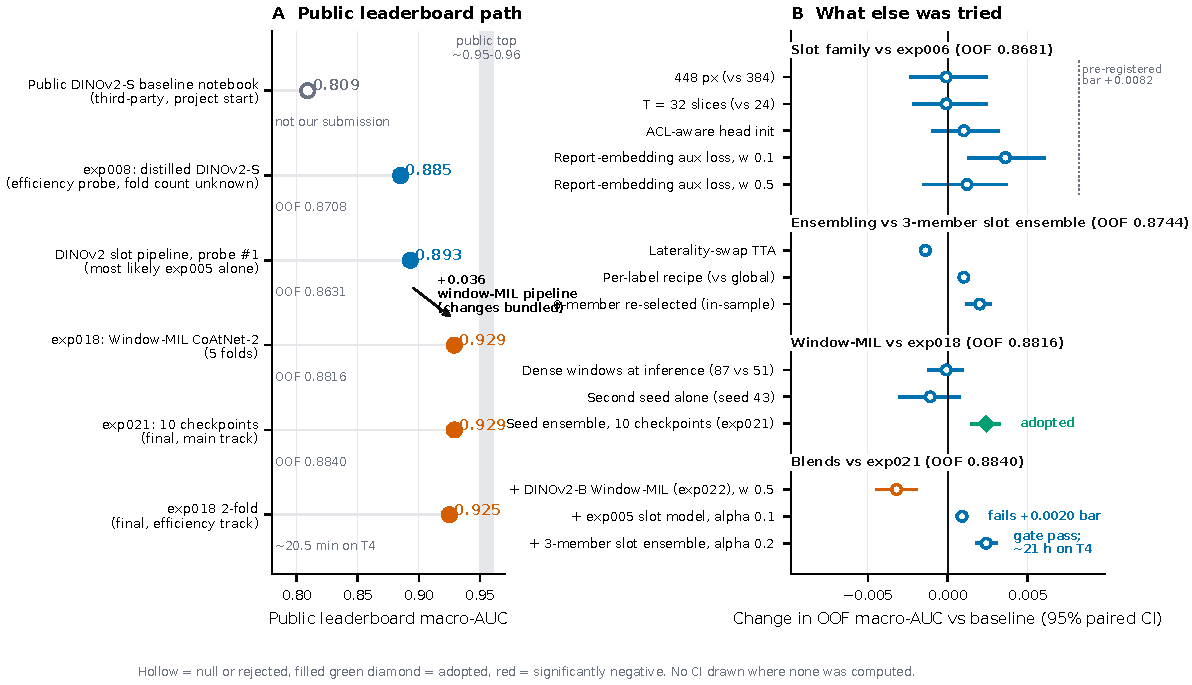
\includegraphics[width=0.93\textwidth]{ablation_path_and_nulls.pdf}
\caption{(A) Public leaderboard path (the 0.809 baseline is a third-party notebook, not a submission). (B) Every tested
change as a paired OOF delta with its 95\% cluster-bootstrap interval, grouped by baseline.}
\label{fig:ablation}
\end{figure*}

\begin{table*}[t]   % PLACEMENT: after Fig. 2; filled from docs/EXPERIMENTS.md (section per row in the SRC comments)
\caption{Ablation ledger. $\Delta$ is OOF macro-AUC against the stated baseline; intervals are paired cluster bootstrap
over 3,681 report clusters unless noted. ``Bar'' is the pre-registered $+0.0082$ for the slot family.}
\label{tab:ablation}
\centering\footnotesize
\begin{tabular}{@{}llccl@{}}
\toprule
Change & Baseline (OOF) & $\Delta$ OOF & 95\% CI & Verdict \\
\midrule
448 px (vs 384) & exp006 (0.8681) & $-0.0001$ & [$-0.0024$, $+0.0025$] & null \\          % SRC: ledger C, exp015
$T=32$ slices (vs 24) & exp006 & $-0.0001$ & [$-0.0022$, $+0.0025$] & null \\              % SRC: ledger C, exp010
ACL-aware head init & exp006 & $+0.0010$ & [$-0.0010$, $+0.0032$] & null (MCL $-0.0122$) \\ % SRC: 2026-09-20 block, exp012
Report-embedding aux loss, $w=0.1$ & exp006 & $+0.0036$ & [$+0.0012$, $+0.0061$] & below bar \\ % SRC: ledger C, exp016a
Report-embedding aux loss, $w=0.5$ & exp006 & $+0.0012$ & [$-0.0016$, $+0.0037$] & null \\ % SRC: ledger C, exp016b
Laterality-swap TTA & 3-member (0.8744) & $-0.0014$ & --- & rejected \\               % SRC: ledger D
Per-label ensemble recipe & 3-member & $+0.0010$ & --- & below $0.002$ bar \\          % SRC: ledger D
6-member re-selected ensemble & 3-member & $+0.0020$ & [$+0.0011$, $+0.0027$] & in-sample; $2.9\times$ cost \\ % SRC: ledger D
Dense windows at inference (87 vs 51) & exp018 (0.8816) & $-0.0001$ & [$-0.0013$, $+0.0010$] & null \\ % SRC: 2026-09-26 dense
Second seed alone (seed 43) & exp018 & $-0.0011$ & [$-0.0031$, $+0.0008$] & null \\       % SRC: 2026-09-25 exp021
\textbf{10-checkpoint seed ensemble} & exp018 & $+0.0024$ & [$+0.0014$, $+0.0033$] & \textbf{adopted} \\ % SRC: 2026-09-25
DINOv2-B inside the window pipeline (solo) & exp018 & $-0.0107$ & --- & worse (0.8709) \\ % SRC: 2026-09-26 exp022; delta = 0.8709-0.8816
EMA, decay 0.999 (fold 0, gold-58) & top-3 average & $-0.0009$ & --- & null \\         % SRC: 2026-09-24 exp020 (fold-0 gold-58, not OOF)
+ DINOv2-B window model, $w=0.5$ & exp021 (0.8840) & $-0.0032$ & [$-0.0045$, $-0.0019$] & gate fail \\ % SRC: 2026-09-26 exp022
+ 3-member slot ensemble, $\alpha=0.2$ & exp021 & $+0.0024$ & [$+0.0017$, $+0.0031$] & gate pass; $\sim$21 h on T4 \\ % SRC: 2026-09-26 gate
+ exp005, $\alpha=0.1$ & exp021 & $+0.0009$ & [$+0.0005$, $+0.0012$] & below $+0.0020$ bar \\ % SRC: 2026-10-01 re-gate
\bottomrule
\end{tabular}
\end{table*}
\begin{notes}
\begin{itemize}
\item \nt{Write the null-result paragraph: six pre-registered slot-family changes inside noise; ViT-S$\to$ViT-B
($+0.005$), v3 labels ($+0.014$) and ensembling ($+0.006$) were the only early gains; the plateau was a property of
the model family.}  % SRC: ledger "Reading the whole record"
\item \nt{Other rejected items worth one clause: DINOv3-S ($-0.0252$), ConvNeXt-V2 (redundant, corr 0.93), 3D ResNet
(killed), CoAtNet-3 (no result: no pretrained checkpoint at the intended size, then a 32-bit indexing overflow).}
  % SRC: ledger B; 2026-09-24
\item \nt{The blend: the 3-member arm passes an offline gate but cannot run in time on T4; the single-model arm fails the
bar; modeling closed.}  % SRC: 2026-09-27, 2026-10-01
\end{itemize}
\end{notes}

\begin{table}[t]   % PLACEMENT: column width; numbers generated by scripts/report_tables.py
\caption{Per-label AUC. OOF: 4,349 studies against report-derived labels; gold-58: against image review.}
\label{tab:perlabel}
\centering\footnotesize
\begin{tabular}{@{}lcccc@{}}
\toprule
 & \multicolumn{2}{c}{OOF} & \multicolumn{2}{c}{Gold-58} \\
\cmidrule(lr){2-3}\cmidrule(lr){4-5}
Finding & exp018 & exp021 & exp018 & exp021 \\
\midrule
ACL & 0.852 & 0.857 & 0.983 & 0.979 \\
MCL & 0.904 & 0.904 & 0.859 & 0.875 \\
Medial Meniscus & 0.936 & 0.938 & 0.986 & 0.986 \\
Lateral Meniscus & 0.902 & 0.913 & 0.840 & 0.834 \\
Medial OA & 0.900 & 0.901 & 0.971 & 0.971 \\
Lateral OA & 0.877 & 0.877 & 0.826 & 0.828 \\
PF OA & 0.835 & 0.836 & 0.825 & 0.824 \\
Effusion & 0.899 & 0.901 & 0.981 & 0.978 \\
Synovitis & 0.817 & 0.818 & 0.842 & 0.847 \\
Baker's & 0.887 & 0.891 & 0.984 & 0.986 \\
Contusion & 0.867 & 0.867 & 0.906 & 0.906 \\
Fracture & 0.905 & 0.907 & 0.907 & 0.922 \\
\midrule
Macro & 0.8816 & 0.8840 & 0.9091 & 0.9111
 \\
\bottomrule
\end{tabular}
\end{table}
\begin{notes}
\begin{itemize}
\item \nt{ACL: lowest-ish on OOF (0.857) but 0.979 on gold-58, so the OOF deficit is proxy-label noise.}
  % SRC: table above; EXPERIMENTS.md 2026-09-18 ACL conclusion
\item \nt{Weakest on gold-58: PF OA 0.824, lateral OA 0.828, lateral meniscus 0.834 ($n=58$: wide intervals).}
\end{itemize}
\end{notes}

\ifextrafigs   % optional: ~0.6 page; the per-label table carries the same numbers
\begin{figure*}[t]
\centering
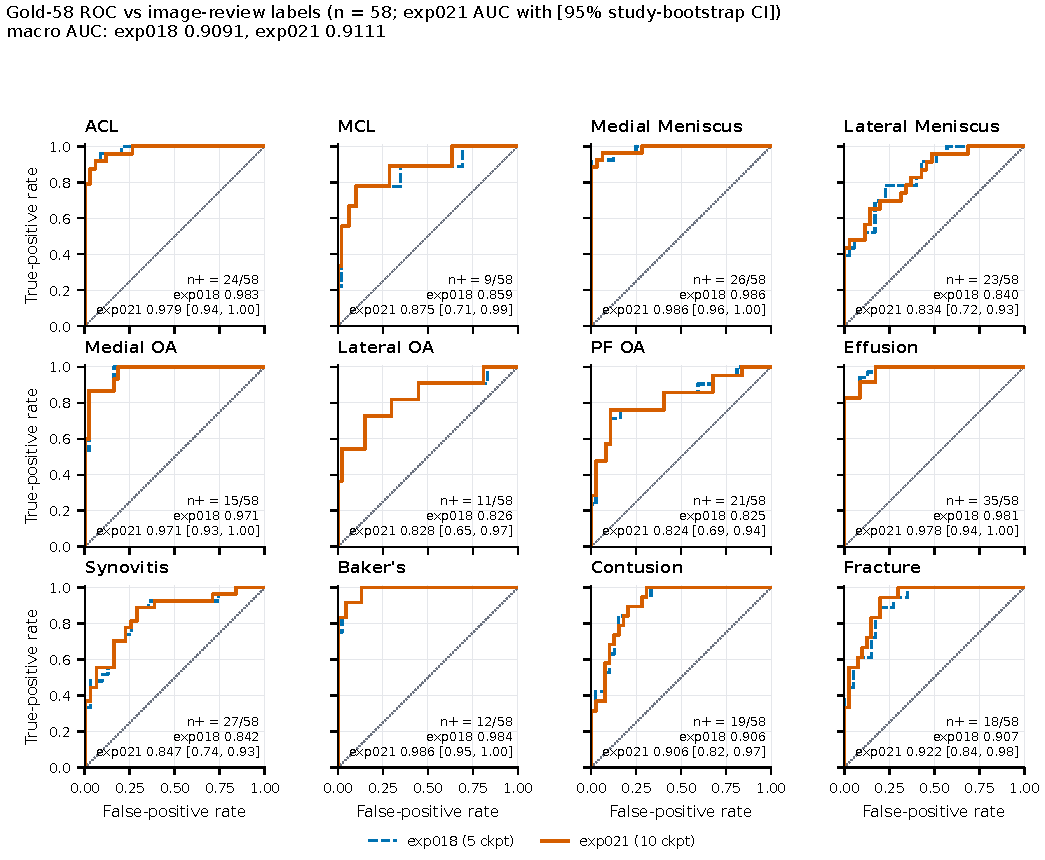
\includegraphics[width=0.93\textwidth]{roc_gold58_exp018_exp021.pdf}
\caption{Per-finding ROC curves on the 58 image-review studies (exp021 AUC with 95\% study-bootstrap interval).}
\label{fig:roc}
\end{figure*}
\begin{figure*}[t]
\centering
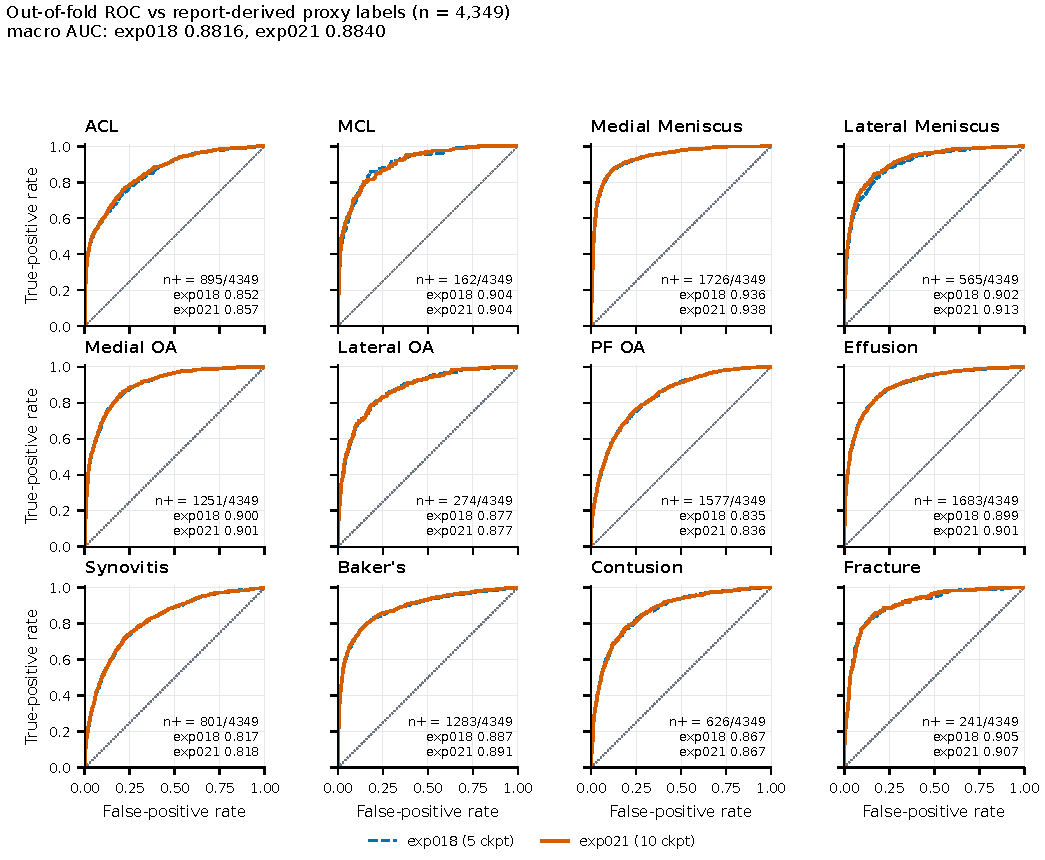
\includegraphics[width=0.93\textwidth]{roc_oof_exp018_exp021.pdf}
\caption{Out-of-fold ROC curves against report-derived labels ($n=4{,}349$).}
\label{fig:rocoof}
\end{figure*}
\fi

\begin{table}[t]
\caption{Efficiency track (maxAUC assumed 0.95; public AUC; lower is better).}
\label{tab:eff}
\centering\footnotesize
\begin{tabular}{@{}lccc@{}}
\toprule
Configuration & LB AUC & Time & Score \\
\midrule
Distilled DINOv2-S & 0.885 & $\sim$11.6 min$^{c}$ & $-1.945$ \\  % SRC: exp018_efficiency_table.md (projected runtime)
Window-MIL, 5 folds & 0.929 & $\sim$53 min & $-1.966$ \\             % SRC: computed: 0.929/(-0.45)+3180/32400
Window-MIL, 2 folds & 0.925 & $\sim$20.5 min & $\mathbf{-2.018}$ \\   % SRC: 2026-09-26 efficiency entries
\bottomrule
\end{tabular}\\[2pt]
{\footnotesize $^{c}$Projected, not measured.}
\end{table}
\begin{notes}
\begin{itemize}
\item \nt{Model-bound, not decode-bound: 5 folds take $\sim$4.5 s/study on one T4 ($\sim$53 min), so fold count is the lever;
2 folds run at the DICOM-decode floor.}  % SRC: 2026-09-26 "C" entries
\item \nt{Tested and not adopted: channels\_last ($-3.7\%$ time, predictions within $3\times10^{-4}$), 4th decode thread (no gain).}
\end{itemize}
\end{notes}

% ======================================================================================================
\section{Analysis}
\begin{figure*}[t]   % PLACEMENT: top of the page; slide variant has 3 rows (the 6-row version is attention_windows_gold58.pdf)
\centering
\includegraphics[width=0.8\textwidth]{attention_windows_gold58_slide.pdf}
\caption{Window-MIL attention (exp021, mean of 10 checkpoints) for three gold-positive studies: the four most-attended
windows and the attention over all windows. Studies were chosen by a fixed rule before any map was viewed (the most
confidently detected gold-positive study per finding); this is a best case, not a hit rate.}
\label{fig:attention}
\end{figure*}
\begin{notes}
\begin{itemize}
\item \nt{Attention view: ACL pools mostly from sagittal fat-suppressed slices, medial meniscus from coronal, Baker's cyst
from axial. Over all 58 gold studies: ACL 62\% of attention on sagittal FS (30\% if uniform), Baker's 45\% on axial (20\%
uniform), effusion 57\% sagittal FS.}  % SRC: docs/figures/attention_slot_mass_gold58.csv
\item \nt{Attention is broad: top-4 windows hold 22--48\% in the selected studies; a finding pools over about 16--40
effective windows (mean 52 windows per study).}  % SRC: same csv, column effective_windows
\item \nt{Caveat: this shows where the pooling draws from, not that it localizes the lesion; no radiologist reviewed the
windows; the two seed groups agree on window attention (per-finding Spearman 0.85--0.95).}  % SRC: csv, seed42_vs_seed43
\end{itemize}
\end{notes}
\ifextrafigs
\begin{figure}[t]
\centering
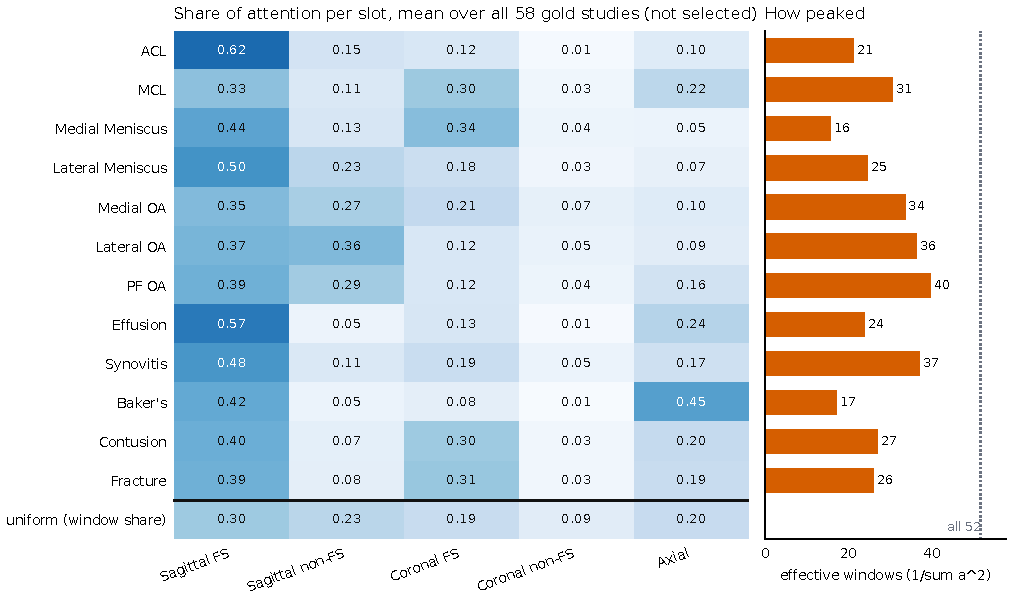
\includegraphics[width=\columnwidth]{attention_by_slot_gold58.pdf}
\caption{Share of attention per slot, all 58 gold studies (not selected), and how peaked the attention is.}
\label{fig:slotshare}
\end{figure}
\fi
\subsection{Validation lessons}
\begin{notes}
\begin{itemize}
\item \nt{OOF vs LB gaps: slot pipeline $\sim-0.030$ (0.8631 vs 0.893; first recorded as $-0.0186$ on the 3-member OOF,
corrected), exp008 $-0.014$ to $-0.020$, exp018 $-0.0474$. Reading: report-derived OOF is a conservative proxy; leakage would
push the other way.}  % SRC: 2026-10-01 correction; METHOD_WRITEUP s11
\item \nt{A runtime degradation ladder silently changed which model was scored: the 3-member notebook measures $\sim$59
s/study on T4 ($\sim$21~h), so it almost certainly ran exp005 alone (inferred, not confirmed). The efficiency notebook also
picked its fold count at run time (unknown). Log the chosen rung; measure on target hardware before trusting a score.}
  % SRC: 2026-09-27, 2026-10-01
\item \nt{Borrowed speed factors were off by 3.6$\times$ (CoAtNet) and $\sim$13$\times$ (DINOv2) between H100 and T4.}
\item \nt{Process lessons worth a sentence each: a ``root cause'' proven off-platform was not on the failing path; a timed join
silently wrote label priors; tests must assert on prediction content, not row counts.}  % SRC: METHOD_WRITEUP s9
\end{itemize}
\end{notes}

\section{Limitations}
\begin{notes}
\begin{itemize}
\item \nt{Gold-58 ($n=58$): 95\% CI about $\pm0.03$ on macro-AUC; differences below $\sim$0.02 cannot be resolved.}
\item \nt{Public leaderboard only; the final private rank is unknown until the competition closes (Oct 22).}
\item \nt{The 0.893 $\rightarrow$ 0.929 gain is not attributed to any single change; attention maps are unvalidated
by a clinician; the 0.893 attribution to exp005 is an inference.}
\item \nt{Label-engine calibration used the same 58 studies that report gold-58 AUC (leave-one-out for the labeler; the image
models never trained on them), so the labeler's own agreement numbers are optimistic.}
\item \nt{No external data; single-person project; Kaggle hardware only for inference.}
\end{itemize}
\end{notes}

\section{Conclusion}
\begin{notes}
\begin{itemize}
\item \nt{Three sentences: what worked (calibrated report labels; per-finding attention over windows; seed ensemble), what
did not (every slot-family lever; blends), and the methodological point (pre-registration, measured runtime, logged
fallbacks).}
\item \nt{Availability: code, weights and write-up to be released after Oct 22 (repository private until then). \todo{insert URL}}
\end{itemize}
\end{notes}

\section*{Acknowledgment}
\nt{Compute: university HPC cluster (H100) and Kaggle T4 notebooks. \todo{add course/instructor thanks}}

\bibliographystyle{IEEEtran}
\bibliography{refs}

\end{document}
